\documentclass[11pt]{article}
\usepackage{graphicx}
\usepackage[T1]{fontenc}
\usepackage[polish]{babel}
\usepackage[utf8]{inputenc}
\usepackage{lmodern}
\usepackage{multirow}
\usepackage{array}
\usepackage{booktabs}
\selectlanguage{polish}
\usepackage{titlesec}
\usepackage{amsmath}
\usepackage{esint}
\usepackage{textpos}
\usepackage{chngpage}
\usepackage{hyperref}
\usepackage{gensymb}
\usepackage{calc}
\usepackage{listings}
\usepackage{placeins}
\titlelabel{\thetitle.\quad}

\begin{document}
\begin{titlepage}
\centering

{\large Wydział Matematyki i Nauk Informacyjnych Politechniki Warszawskiej}

\vspace{1cm}

\includegraphics[scale=0.15]{logo}
\vspace{3cm}

{\Huge\bfseries Sprawozdanie \# 03}
\\
\vspace{.2cm}
{\huge Analiza i Przetwarzanie Obrazów Biometrycznych}
\\
\vspace{.2cm}
{\Large\bfseries Ścienianie - KMM oraz K3M}

\vspace{1cm}

{\Large Tomasz Koter}

\vspace{1cm}

{\large v1.0}

\vspace{1cm}

\vfill

{\itshape {\large 1 gru 2016}}
\end{titlepage}

\tableofcontents
\newpage

\section{Wstęp}
\par
Niniejsze sprawozdanie dotyczy laboratoriów \# 4 oraz \# 5 Analizy i Przetwarzania Obrazów Biometrycznych 2016Z, czyli algorytmów ścieniania KMM oraz K3M. Zadaniem była implementacja obu.
\par
W celu realizacji tego zadania posłużyłem się Octave (na 99\% programy są kompatybilne z  Matlabem) ze względu na wygodę i szybkość obróbki obrazów za jego pomocą. Octave oferuje możliwość prostego przetwarzania całego obrazu za pomocą pojedynczej linii kodu zawierającej jakieś wyrażenie logiczne lub arytmetyczne, dzięki czemu na ogół można uniknąć pisania podwójnych pętli po kolejnych pikselach obrazu lub korzystania z generatorów, co nadal jest dłuższe niż jednolinijkowe wyrażenie. 
\par
Ponadto w podstawowym pakiecie oraz w rozszerzeniu \textit{image} dostępne są przydatne funkcje, takie jak splot czy dodawanie marginesu do obrazu, co ułatwia korzystanie z masek (nie można wyjść poza zakres tablicy obrazu). Są to funkcje dość trywialne do napisania, lecz mimo tego są czasochłonne i zaciemniałyby idee algorytmów swoją objętością.
\par
Oba te algorytmy są świetnie opisane w odpowiadającym im pracach naukowych, o których informacje zamieściłem w sekcji \textit{źródła}. Niemniej opiszę w kolejnej sekcji swój autorski kod i dalej pokażę kilka przykładowych wyników jego działania. Przykłady wyników obu programów umieściłem w jednym rozdziale, żeby łatwiej było porównać je ze sobą. Wszystkie pliki z kodem źródłowym można znaleźć na końcu sprawozdania lub pod \href{https://github.com/caravard/aipob-thinning}{tym adresem}\footnote{https://github.com/caravard/aipob-thinning}.
\par
Implementacja to dwie funkcje w plikach \textit{.m}, przyjmujące na wejściu obraz zbinaryzowany (macierz/tablicę dwuwymiarową), gdzie 0 (czerń) to kolor obiektów, a 1 to kolor tła. Zwracają nowy obraz, bez modyfikacji wejściowego, dlatego nie trzeba martwić się o utratę danych. Do własnych testów, jeśli taka wola czytelnika, wystarczy załadować obraz np. za pomocą \textit{imread}, a po wykonaniu na nim funkcji \textit{KMM} lub \textit{K3M} wyświetlić za pomocą \textit{imshow}.

\section{KMM}

\subsection{Algorytm i implementacja}
\par
Załączona implementacja pozwala wyznaczyć szkielet lub kontur wprowadzonego obrazu, zależnie od przekazanego do funkcji argumentu (opis parametrów znajduje się w pliku funkcji, można też o nich przeczytać za pomocą \textit{help kmm}).
\par
Poniżej przedstawiony kod jest opisany komentarzami w pliku, więc nie będę opisywał tutaj każdego fragmentu kodu osobno. Przedstawię jedynie algorytm, według którego jest napisany - czyli przedstawię moją interpretację opisu w źródłach. Sam algorytm wykorzystuje strategię "palenia trawy", to znaczy iteracyjnie usuwa kontur obiektu do momentu uzyskania szkieletu.
\par
Program przyjmuje na wejściu obraz zbinaryzowany, gdzie 0 (czerń) to kolor obiektu, 1 (biel) to kolor tła. Następnie odwraca kolory tego obrazu, by tło miało wartość 0, a obiekt 1. Potem wchodzi w główną pętlę algorytmu, stanowiącą jego ciało:
\begin{enumerate}
\item Zaznacz kontur obiektu za pomocą \textit{2}
\item Spośród pikseli konturu zaznacz na podstawie wag "łokcie" za pomocą \textit{3}
\item Zaznacz piksele konturu, które mają 2, 3 lub 4 przylegających do siebie sąsiadów za pomocą \textit{4}
\item Usuń wszystkie \textit{4}
\item Dla każdego piksela, który jest oznaczony jako \textit{2}:
	\begin{enumerate}
	\item Oblicz jego wagę
	\item Jeśli ta waga jest w stablicowana jako do usunięcia, ustaw ten piksel jako 0, wpp. jako 1
	\end{enumerate}
\item Dla każdego piksela, który jest oznaczony jako \textit{3}:
	\begin{enumerate}
	\item Oblicz jego wagę
	\item Jeśli ta waga jest w stablicowana jako waga piksela do usunięcia, ustaw ten piksel jako 0, wpp. jako 1
	\end{enumerate} 
\item Jeśli nastąpiła jakaś zmiana, wykonaj pętlę jeszcze raz. Wpp. zakończ działanie
\end{enumerate}
Ostatecznie otrzymany obraz znów odwracamy, by był w tej samej palecie barw, co przed uruchomieniem programu.
\par
Oczywiście rodzi się kilka pytań, to znaczy jak zaznaczyć kontur, o co chodzi z wagami oraz o co chodzi z tablicą wag pikseli do usunięcia.
\par
Waga piksela to nic innego jak liczba binarna, oznaczająca które z pikseli w 8-sąsiedztwie rozważanego pisela obiektu również należy do obiektu. Skoro takich pikseli może być maksymalnie 8, to będzie to wartość z przedziału \textit{\{0, ..., 255\}}. W mojej implementacji oblicza się ją za pomocą splotu obrazu z poniższą maską oraz wyzerowanie przypadkowo obliczonych wag dla pikseli tła.
\[ \begin{bmatrix}
128 & 1 & 2 \\
64 & 0 & 4 \\
32 & 16 & 8
\end{bmatrix} = \begin{bmatrix}
1000\,0000 & 0000\,0001 & 0000\,0010 \\
0100\,0000 & 0000\,0000 & 0000\,0100 \\
0010\,0000 & 0001\,0000 & 0000\,1000
\end{bmatrix}\]
\par
Jak widać, kontur będą stanowić wszystkie te piksele, dla których obliczona waga jest różna od \textit{0} (tło) i od \textit{255} (piksel obiektu nie sąsiadujący z tłem). Przyjmujemy, że jednopikselowe elementy obiektu, tzn. takie piksele, które należą do obiektu i nie posiadają żadnych sąsiadów należących do obiektów, nie istnieją (bo algorytm oczekuje 8-spójnych obiektów), a jeśli nawet by istniały, to nie dałoby się ich ścienić, bo są maksymalnie zredukowane.
\par
Stąd powinno być jasne, że stablicowane są pewne konfiguracje ułożeń sąsiadów, które oznaczają, że usunięcie danego piksela jest bezpieczne dla struktury obrazu i przyczyni się ku stworzeniu szkieletu. Autorzy algorytmu twierdzą, że te konfiguracje zostały wyznaczone empirycznie dla uzyskania efektów najbardziej pożądanych.



\section{K3M}

\subsection{Algorytm i implementacja}
\par
Implementacja tego algorytmu nie pozwala wyznaczyć samego konturu obrazu, gdyż robi to już implementacja KMM. Poza tym korzystanie z funkcji K3M wygląda tak samo. Zanim czytelnik przeczyta tę część sprawozdania, należy zapoznać się z rozdziałem dotyczącym KMM, gdyż duża część metod tam opisanych jest ponownie wykorzystana w K3M.
\par
K3M jest ulepszonym i bardziej usystematyzowanym algorytmem KMM. W jego skład wchodzi siedem logicznie wyodrębnionych faz. To tak samo jak KMM algorytm iteracyjny typu "palenia trawy".
\par
Wyżej wspomniane fazy ustalają, które piksele obiektu należy zamienić na piksele tła. Pierwszych sześć faz jest powtarzanych iteracyjnie do momentu, gdy w ciągu jednego powtórzenia nie nastąpi żadna zmiana w obrazie. Sposób, w jaki usuwane są piksele, może pozostawić w pewnych miejscach drobne dwupikselowe zgrubienia, dlatego na zakończenie wykonania algorytmu, już poza pętlą, wykonuje się operacje ostatniej fazy, by pozostawić szkielet o grubości jednego piksela.
\par
Poszczególne fazy opisane są następująco: \\
\textbf{Faza 0:} Oznaczanie konturu - w taki sam sposób jak w KMM oznaczony zostaje kontur (w implementacji jako \textit{2}). \\
\textbf{Faza 1:} Usunięcie pikseli konturu z 3 przylegającymi do siebie sąsiadami. \\
\textbf{Faza 2:} Usunięcie pikseli konturu z 3 lub 4 przylegającymi do siebie sąsiadami. \\
\textbf{Faza 3:} Usunięcie pikseli konturu z 3, 4 lub 5 przylegającymi do siebie sąsiadami. \\
\textbf{Faza 4:} Usunięcie pikseli konturu z 3, 4, 5 lub 6 przylegającymi do siebie sąsiadami. \\
\textbf{Faza 5:} Usunięcie pikseli konturu z 3, 4, 5, 6 lub 7 przylegającymi do siebie sąsiadami. \\
\textbf{Faza 6:} Usunięcie zgrubień na szkielecie za pomocą dodatkowej tablicy wag. \\
Wszystkie wagi pikseli o powyżej podanych konfiguracjach sąsiadów są stablicowane ze względów optymalizacyjnych.

\section{Przykłady}

\par
Chciałbym przedstawić wyniki dla kilku rodzajów obrazów: prymitywów: prostokąta, koła, pierścienia; plamy z wypustkami, małego obrazka oraz pisma maszynowego i odręcznego.

\begin{figure}[!ht] 
  \caption{Prostokąt}
  \label{ fig7} 
  \begin{minipage}[b]{0.5\linewidth}
    \centering
    
\includegraphics[width=.5\linewidth]{../images/rectangle} 
    \caption{Obraz wejściowy} 
    \vspace{4ex}
  \end{minipage}%%
  \begin{minipage}[b]{0.5\linewidth}
    \centering
    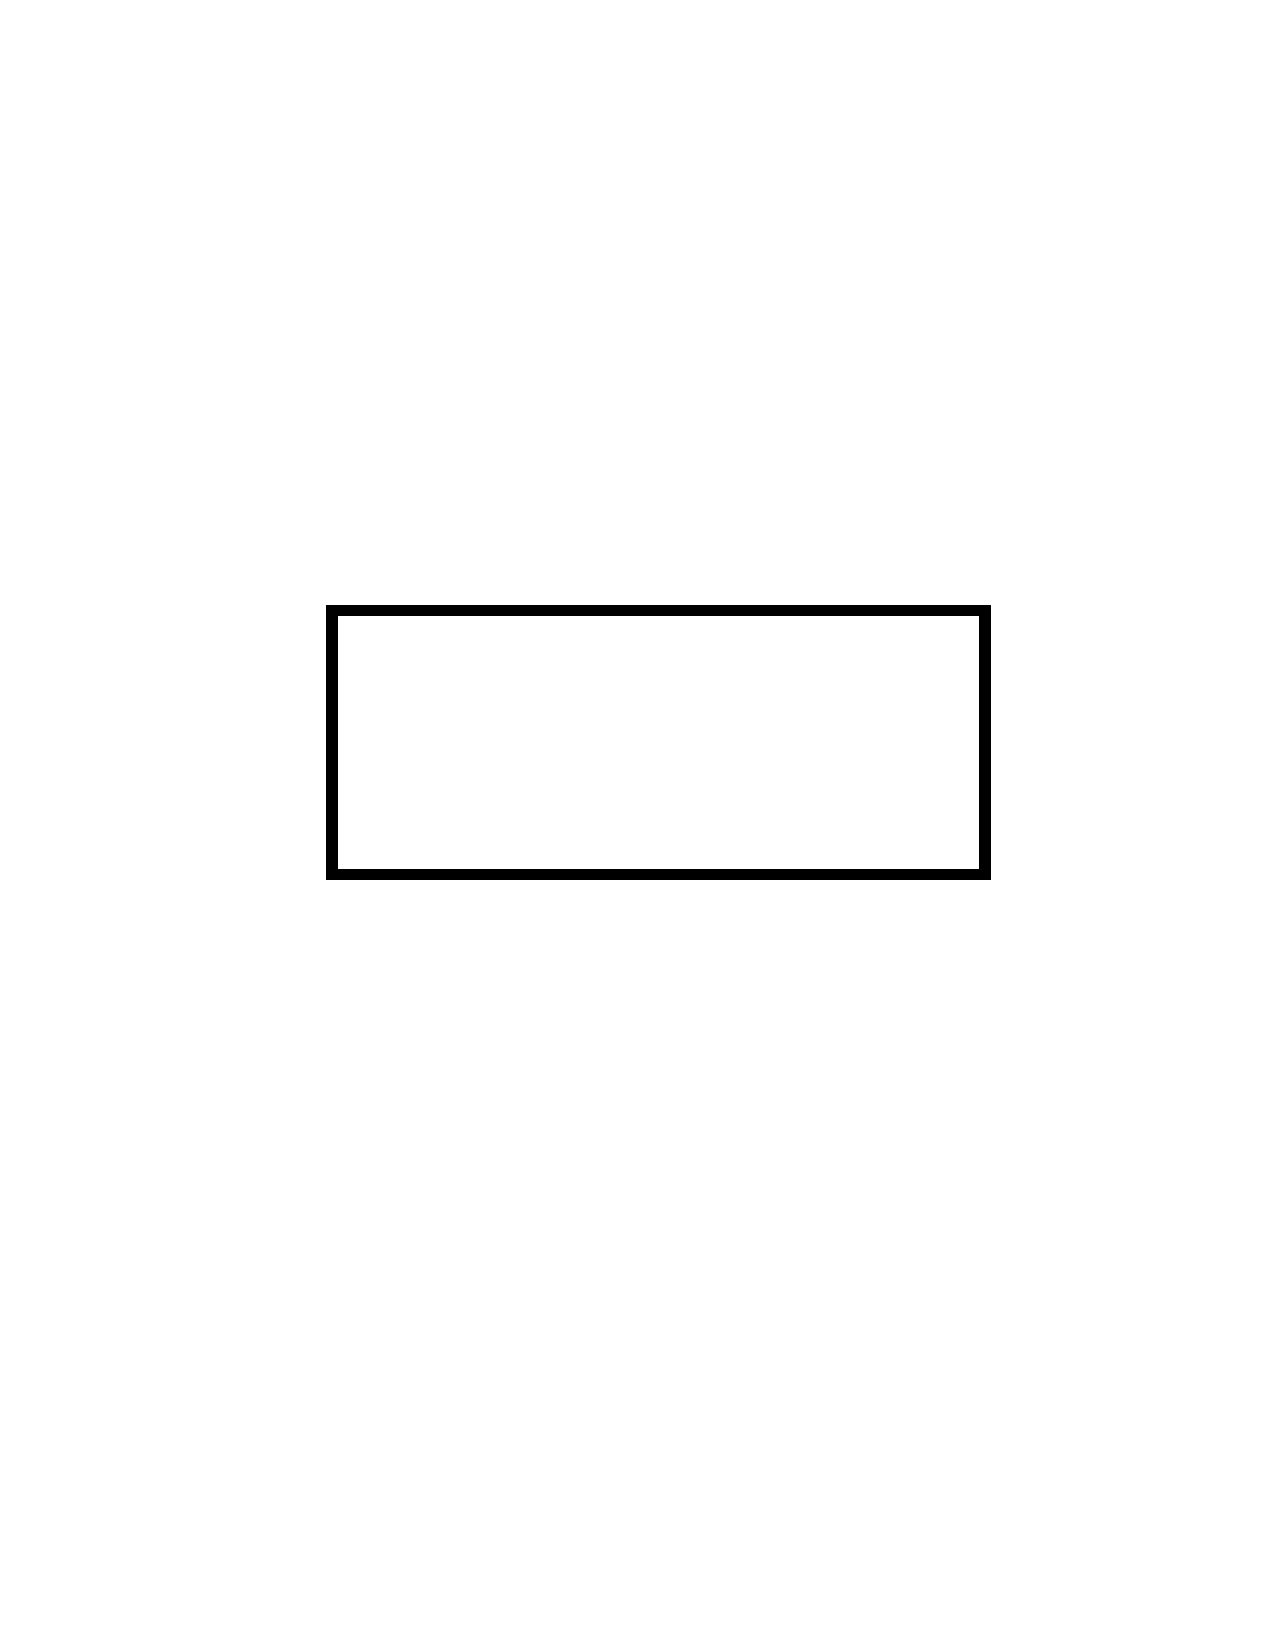
\includegraphics[width=.5\linewidth]{../samples/rect_kmm_contour} 
    \caption{KMM - kontur} 
    \vspace{4ex}
  \end{minipage} 
  \begin{minipage}[b]{0.5\linewidth}
    \centering
    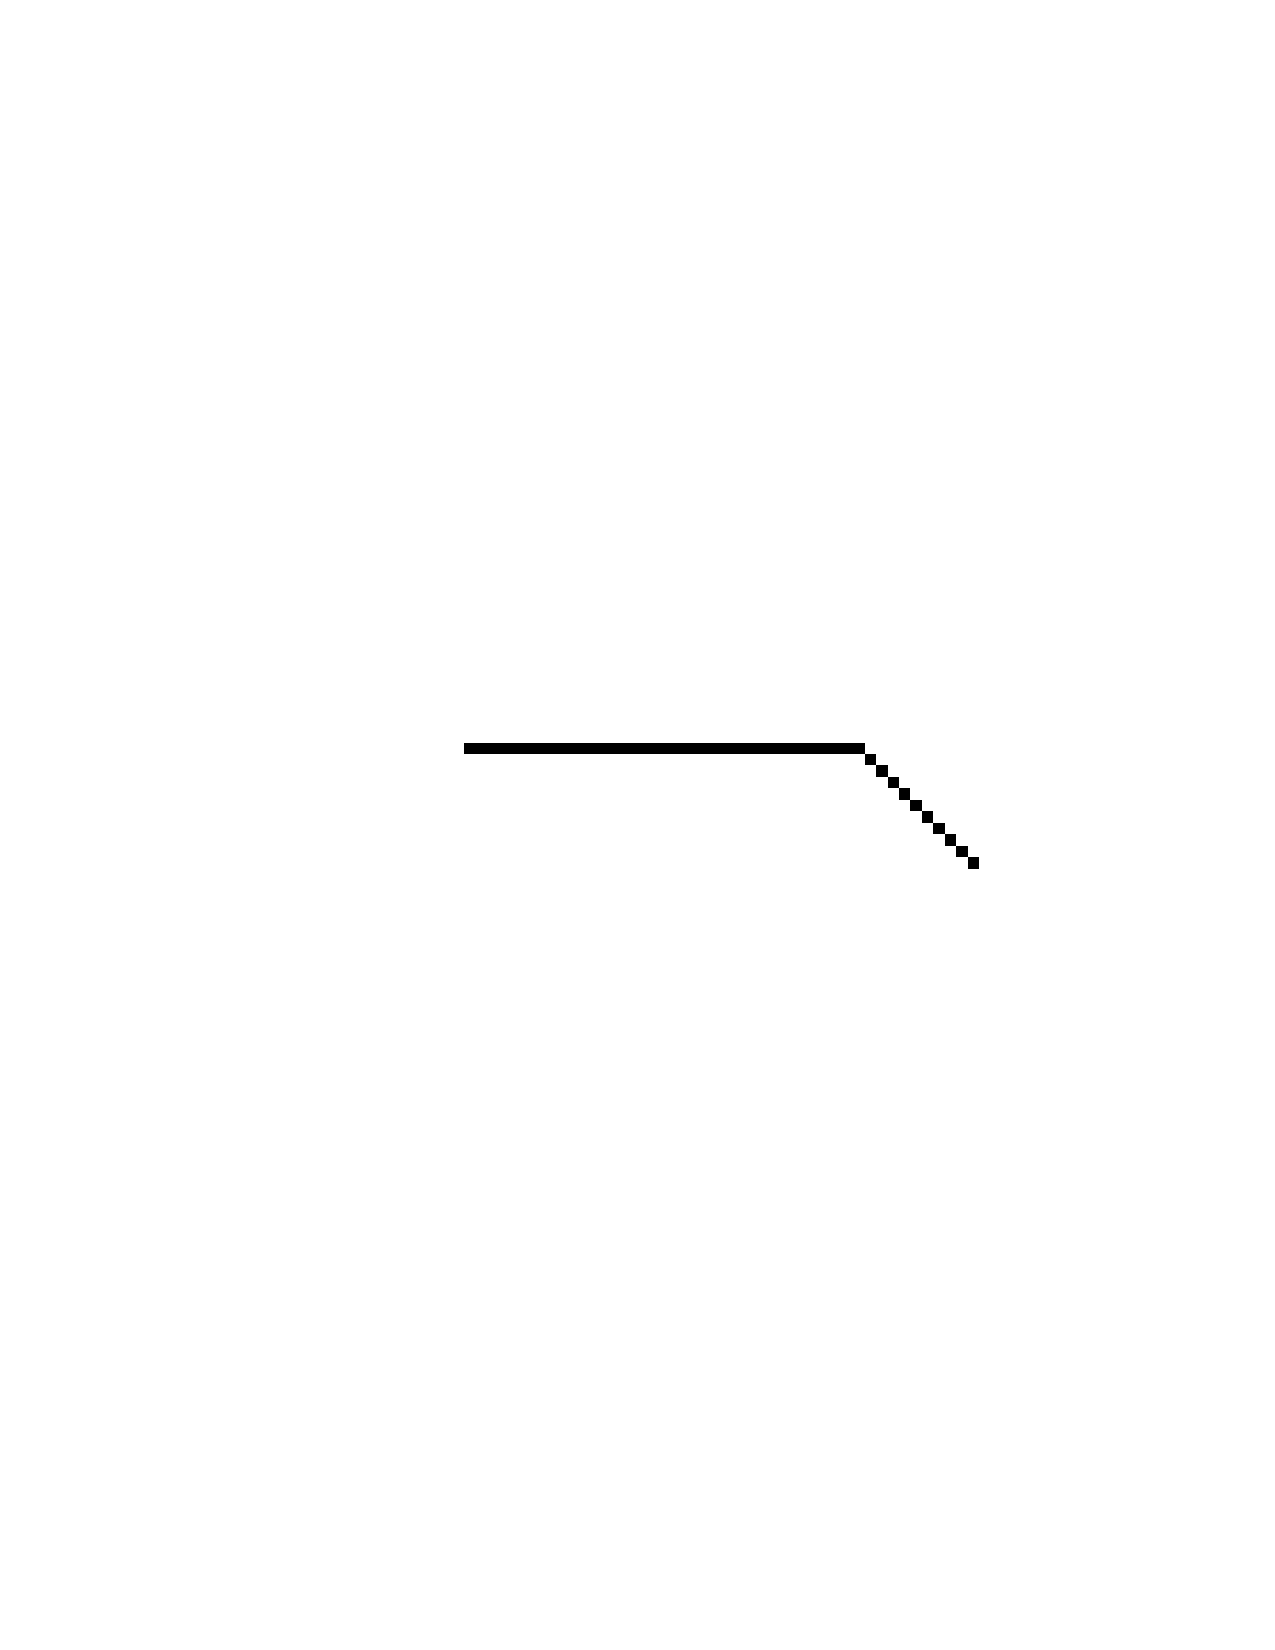
\includegraphics[width=.5\linewidth]{../samples/rect_kmm} 
    \caption{KMM} 
    \vspace{4ex}
  \end{minipage}%% 
  \begin{minipage}[b]{0.5\linewidth}
    \centering
    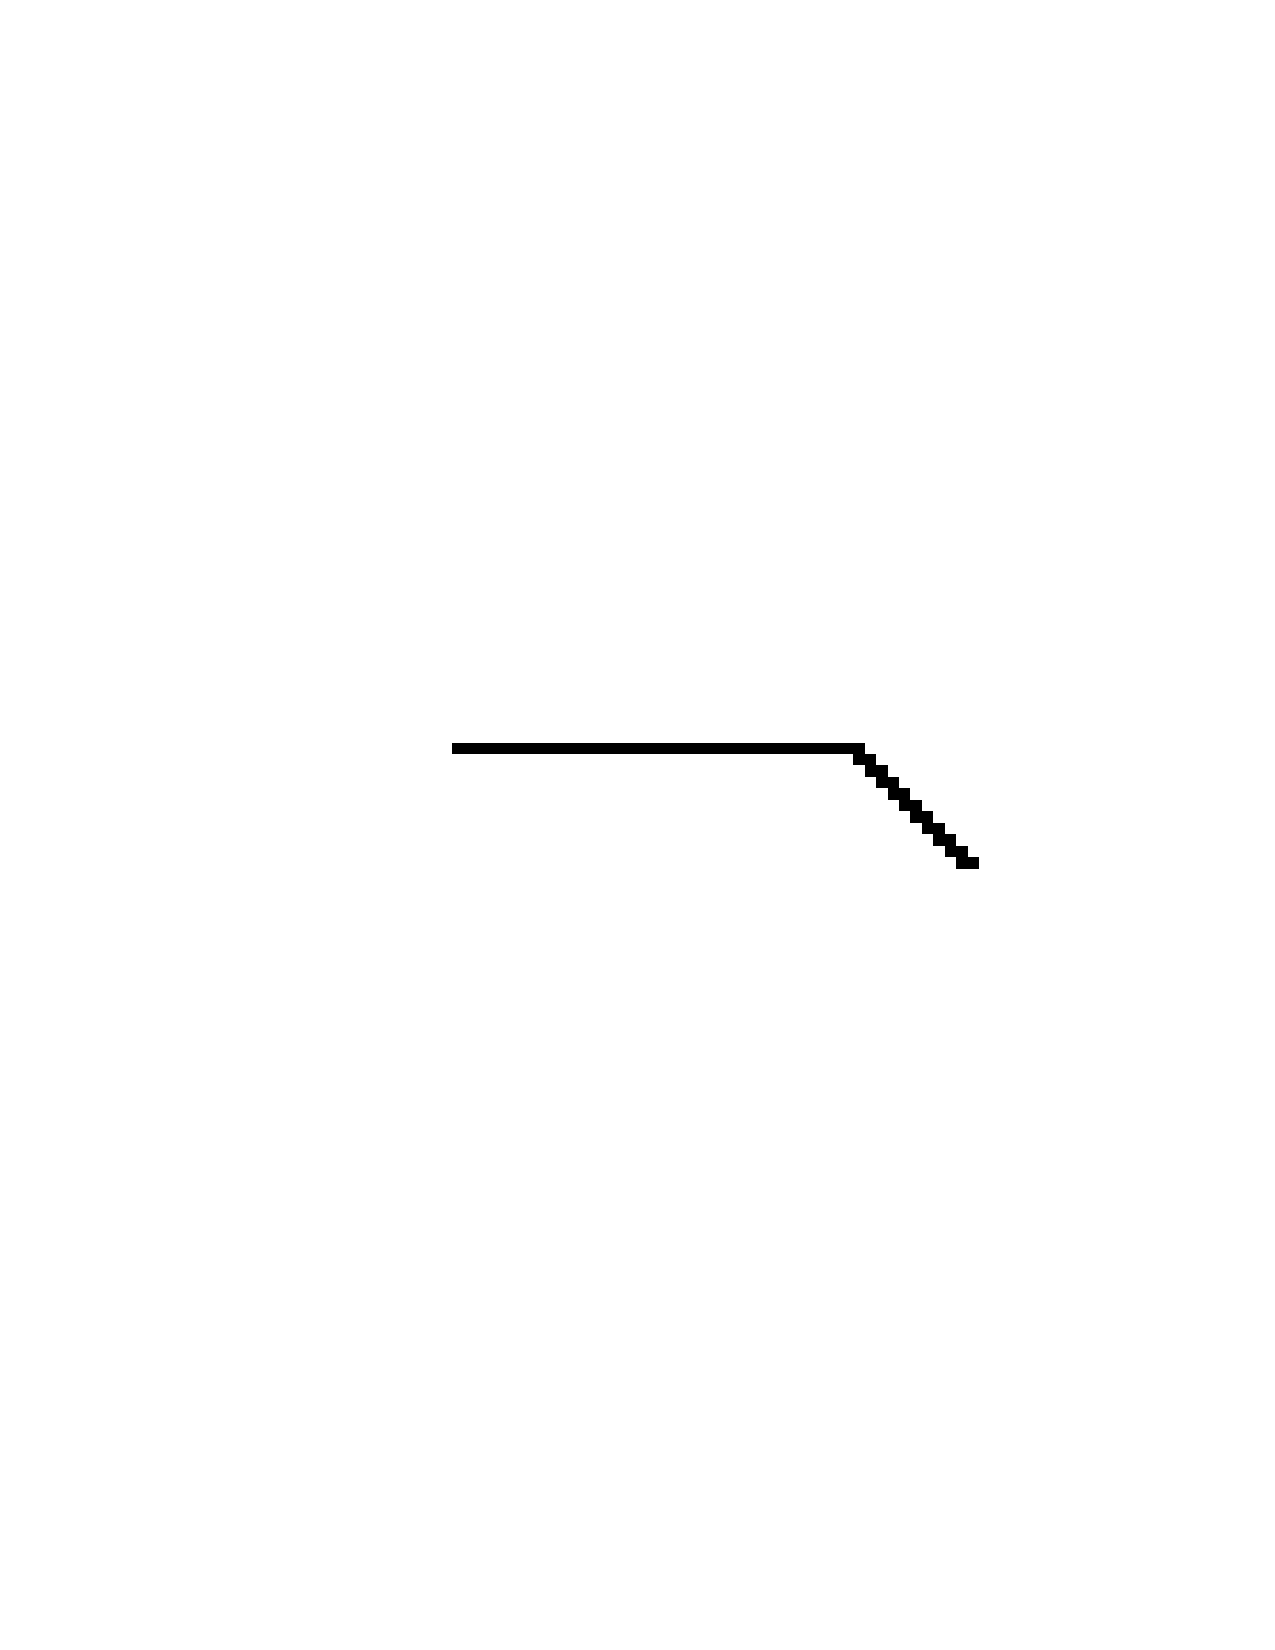
\includegraphics[width=.5\linewidth]{../samples/rect_k3m} 
    \caption{K3M} 
    \vspace{4ex}
  \end{minipage} 
\end{figure}
\FloatBarrier

\begin{figure}[!ht] 
  \caption{Koło}
  \label{ fig7} 
  \begin{minipage}[b]{0.5\linewidth}
    \centering
    
\includegraphics[width=.5\linewidth]{../images/circle} 
    \caption{Obraz wejściowy} 
    \vspace{4ex}
  \end{minipage}%%
  \begin{minipage}[b]{0.5\linewidth}
    \centering
    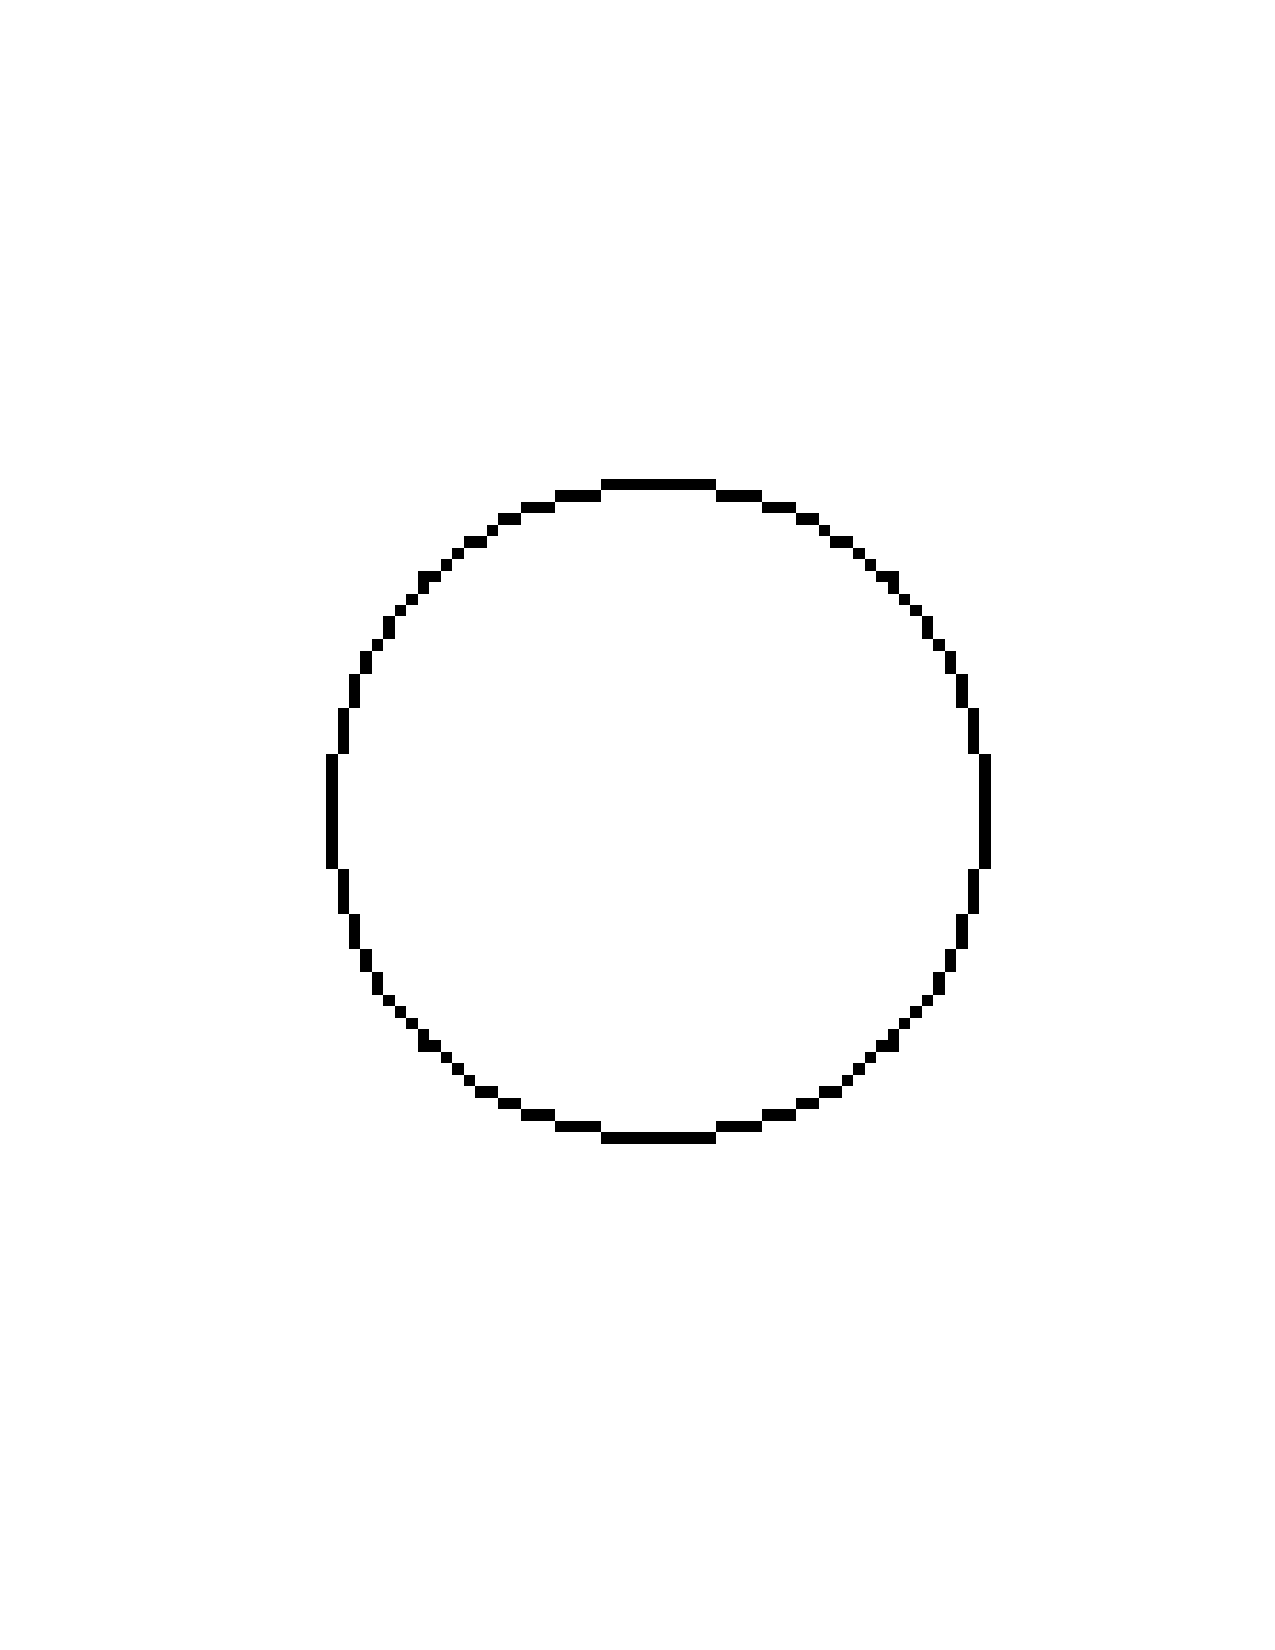
\includegraphics[width=.5\linewidth]{../samples/circle_kmm_contour} 
    \caption{KMM - kontur} 
    \vspace{4ex}
  \end{minipage} 
  \begin{minipage}[b]{0.5\linewidth}
    \centering
    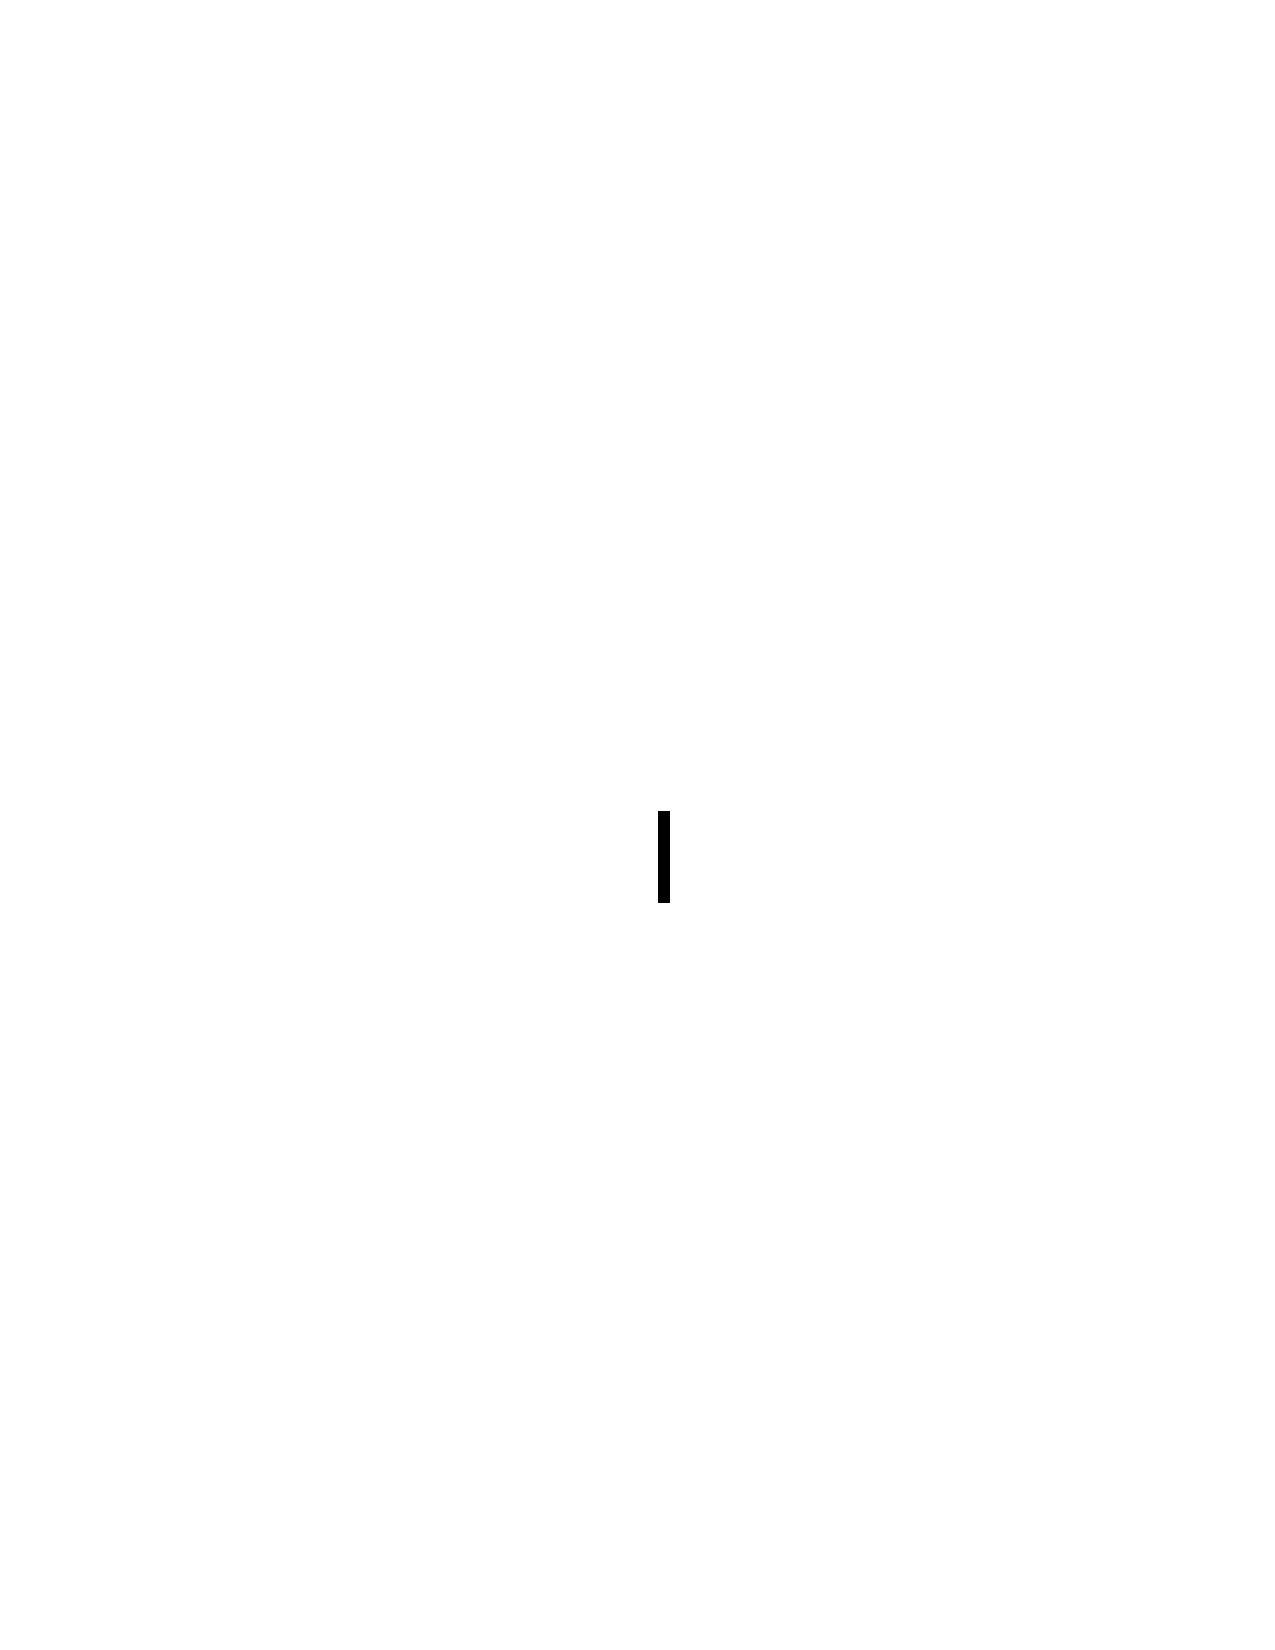
\includegraphics[width=.5\linewidth]{../samples/circle_kmm} 
    \caption{KMM} 
    \vspace{4ex}
  \end{minipage}%% 
  \begin{minipage}[b]{0.5\linewidth}
    \centering
    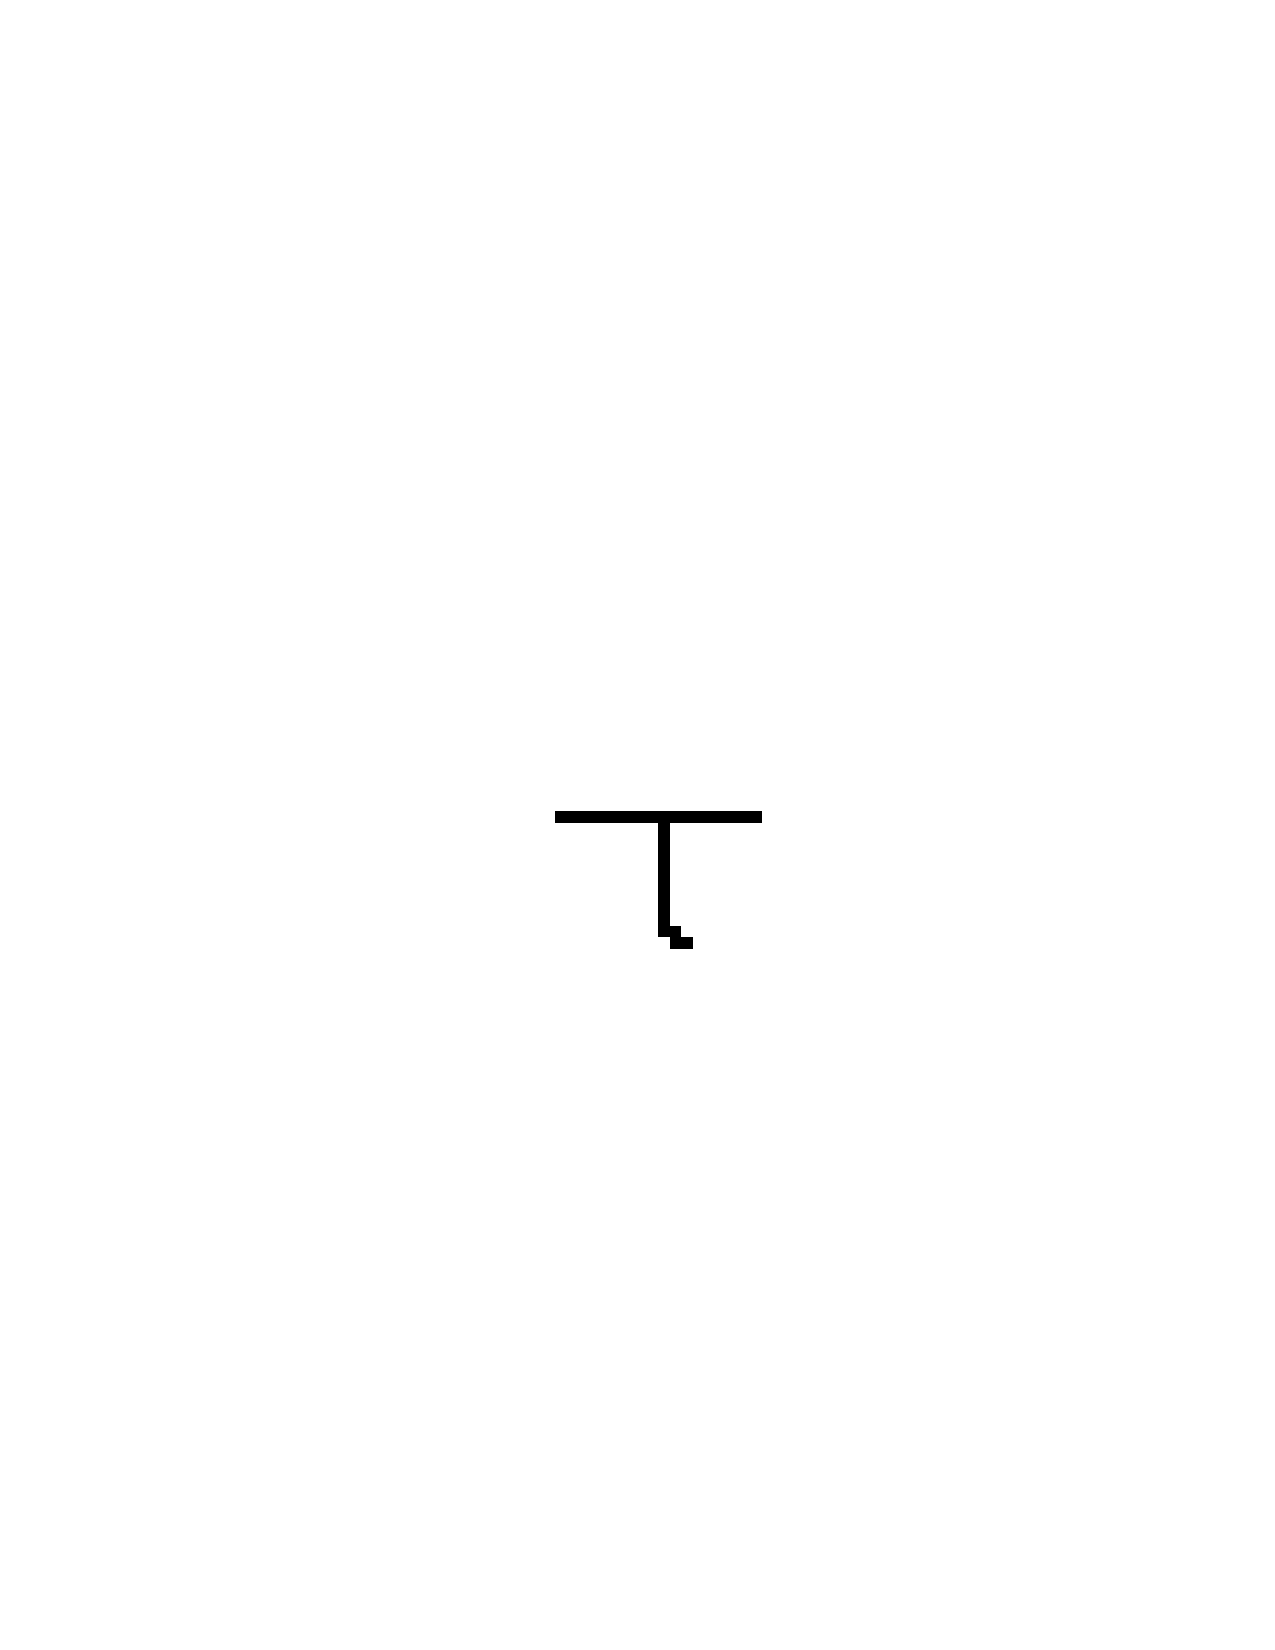
\includegraphics[width=.5\linewidth]{../samples/circle_k3m} 
    \caption{K3M} 
    \vspace{4ex}
  \end{minipage} 
\end{figure}
\FloatBarrier

\par
Jak widać na tych dwóch przykładach, dla prostokąta czy koła bardzo trudno zdefiniować szkielet w ten sposób. W końcu nie wiadomo, czy powinien to być po prostu punkt, czy ten szkielet powinien rozpinać figurę, czy w wypadku prostokąta może odcinek równoległy do dłuższego boku. Stąd biorą się dziwne kształty wynikowych szkieletów - w wypadku koła dla K3M mieszanka próby rozpięcia figury ze zbiegnięciem się do punktu, dla prostokąta coś między rozpięciem figury a odcinkiem. Jak się potem okaże, K3M ma tendencję do zachowywania linii pod kątem 135\degree.

\begin{figure}[!ht] 
  \caption{Pierścień}
  \label{ fig7} 
  \begin{minipage}[b]{0.5\linewidth}
    \centering
    
\includegraphics[width=.5\linewidth]{../images/ring} 
    \caption{Obraz wejściowy} 
    \vspace{4ex}
  \end{minipage}%%
  \begin{minipage}[b]{0.5\linewidth}
    \centering
    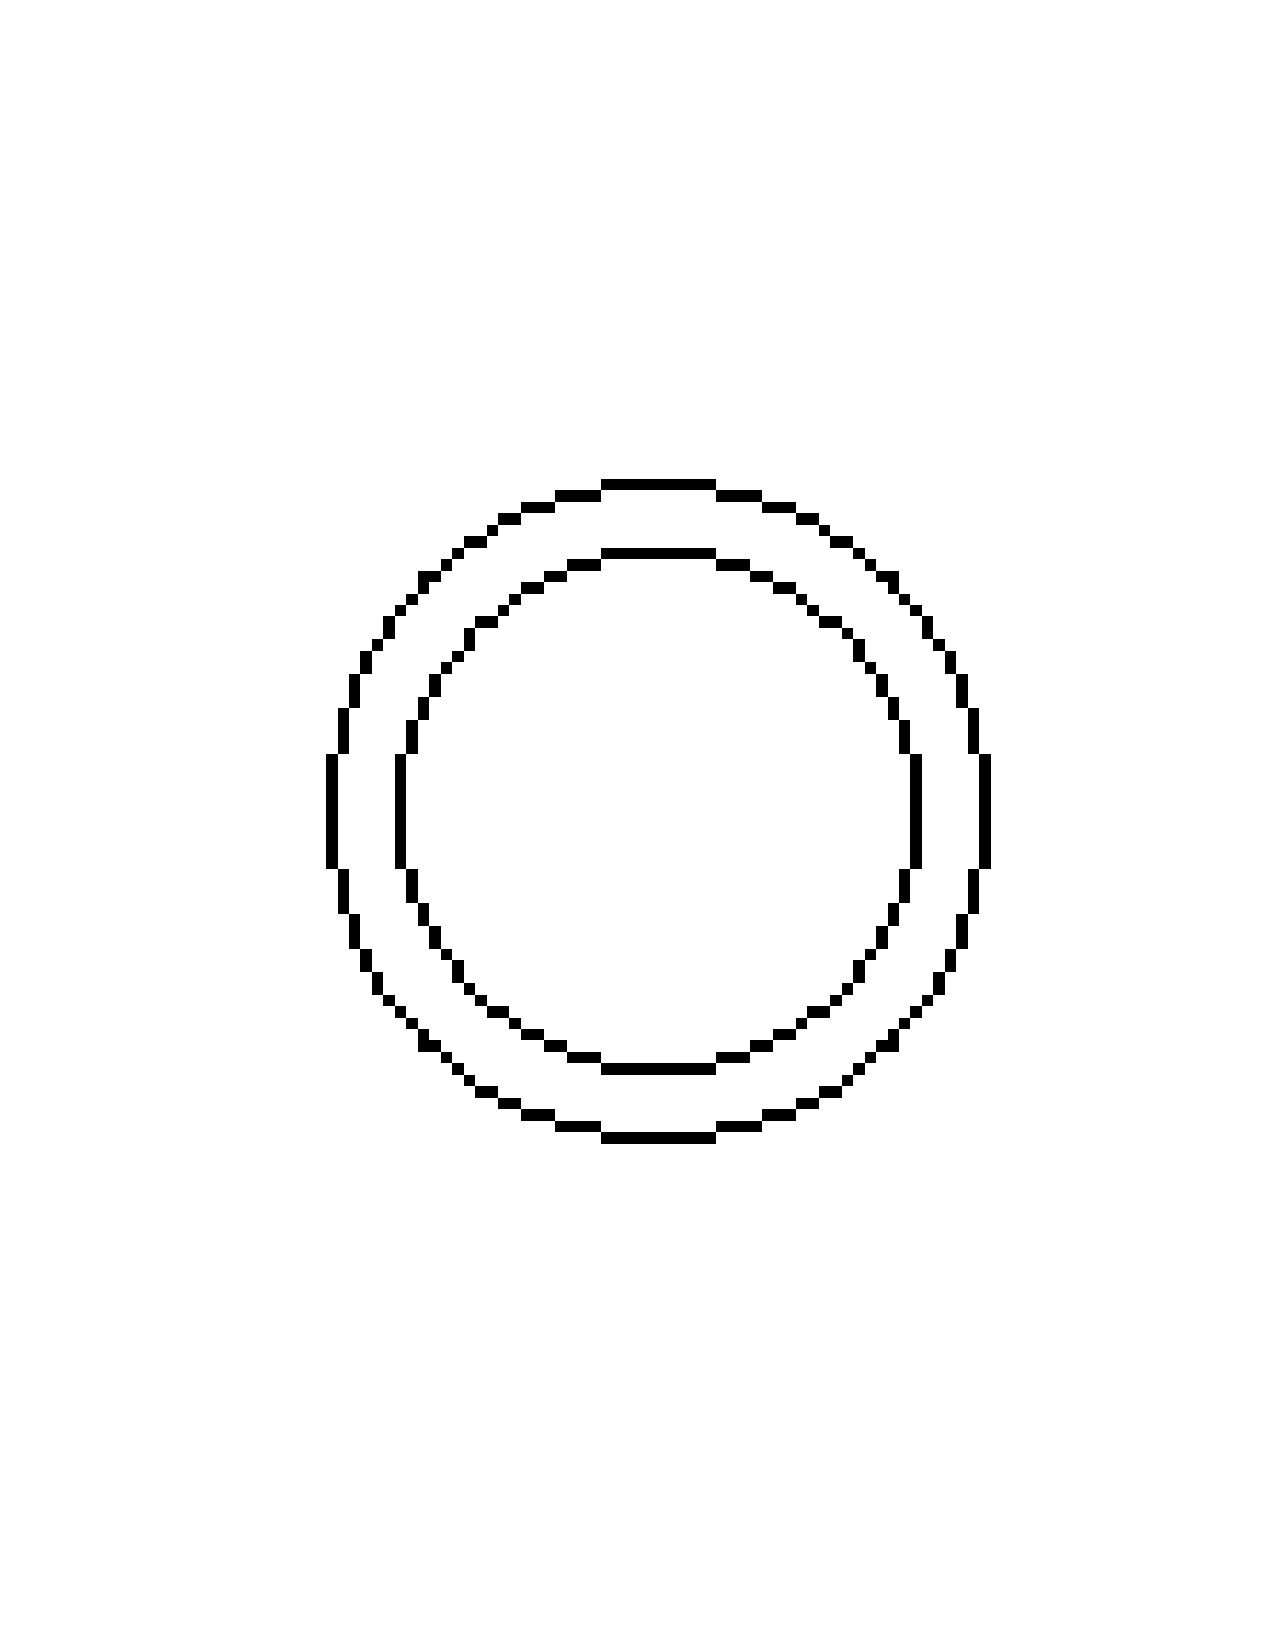
\includegraphics[width=.5\linewidth]{../samples/ring_kmm_contour} 
    \caption{KMM - kontur} 
    \vspace{4ex}
  \end{minipage} 
  \begin{minipage}[b]{0.5\linewidth}
    \centering
    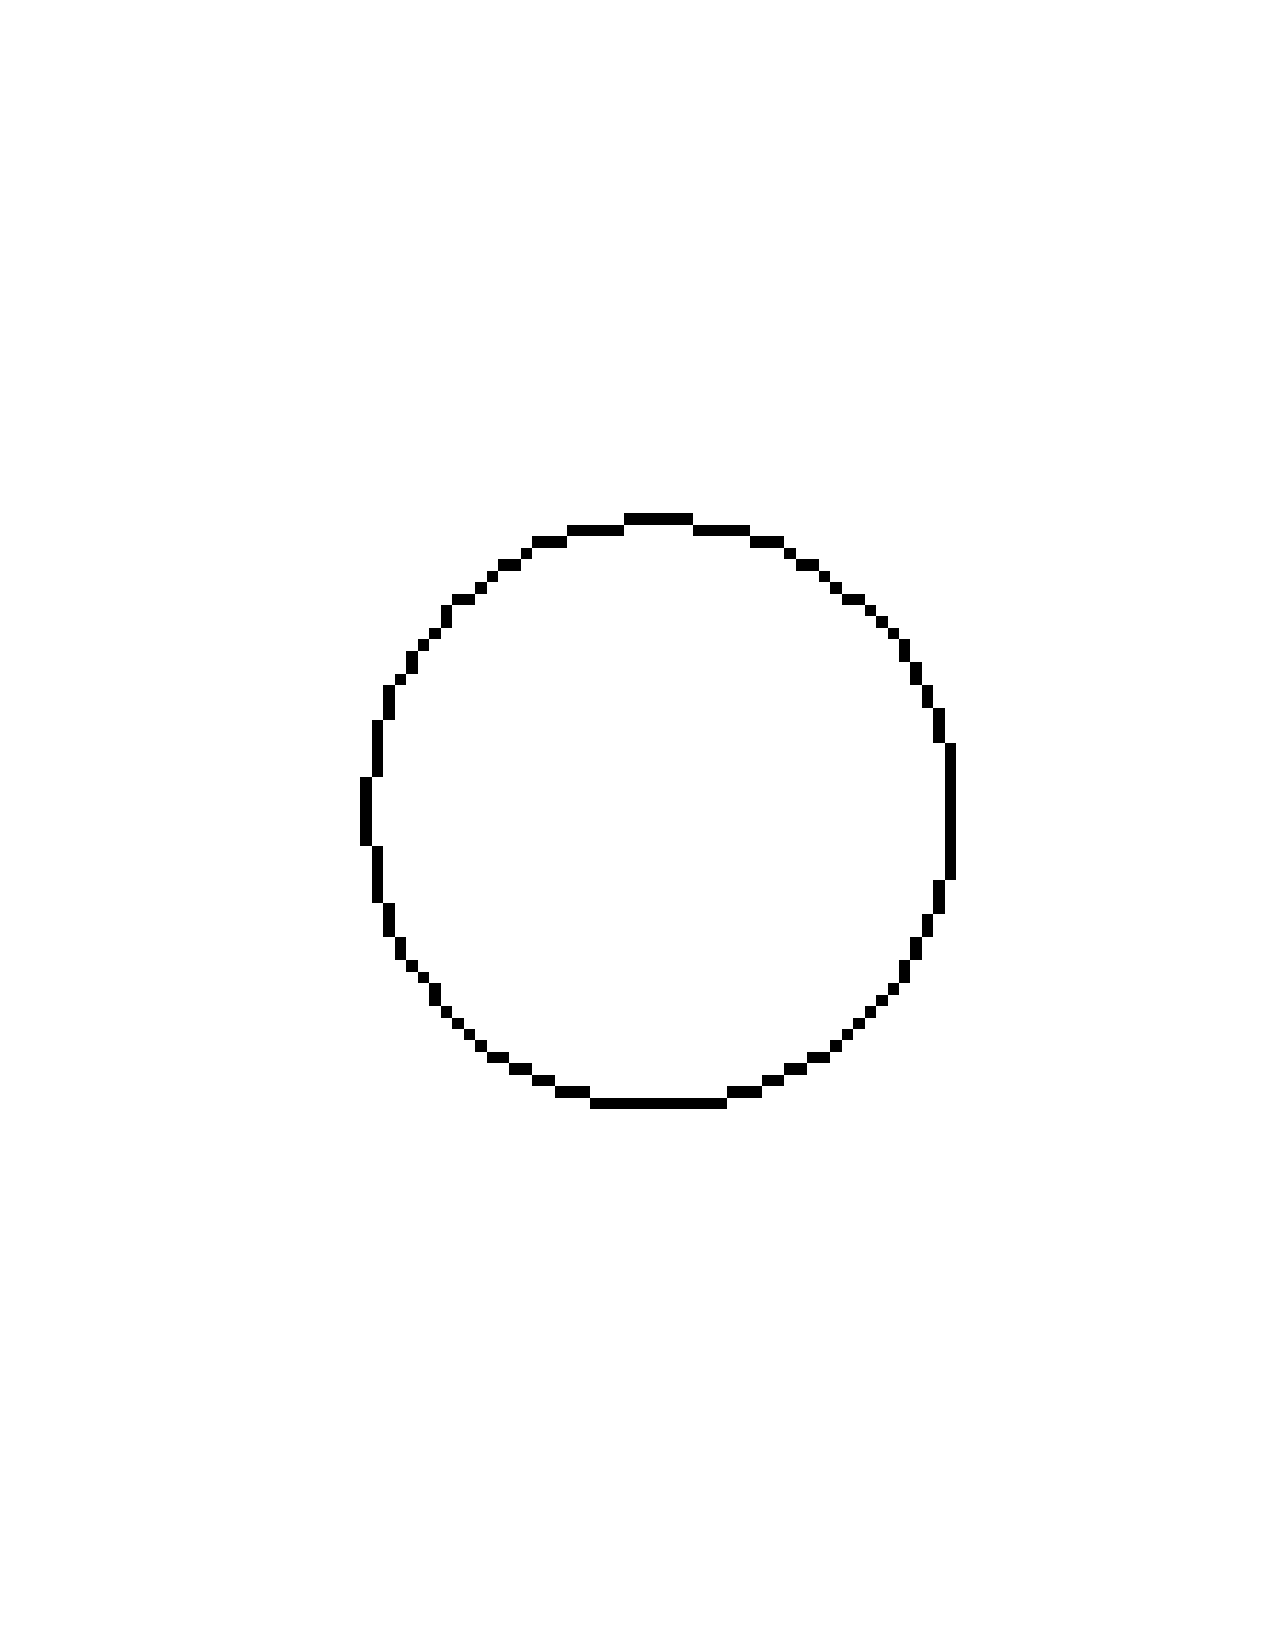
\includegraphics[width=.5\linewidth]{../samples/ring_kmm} 
    \caption{KMM} 
    \vspace{4ex}
  \end{minipage}%% 
  \begin{minipage}[b]{0.5\linewidth}
    \centering
    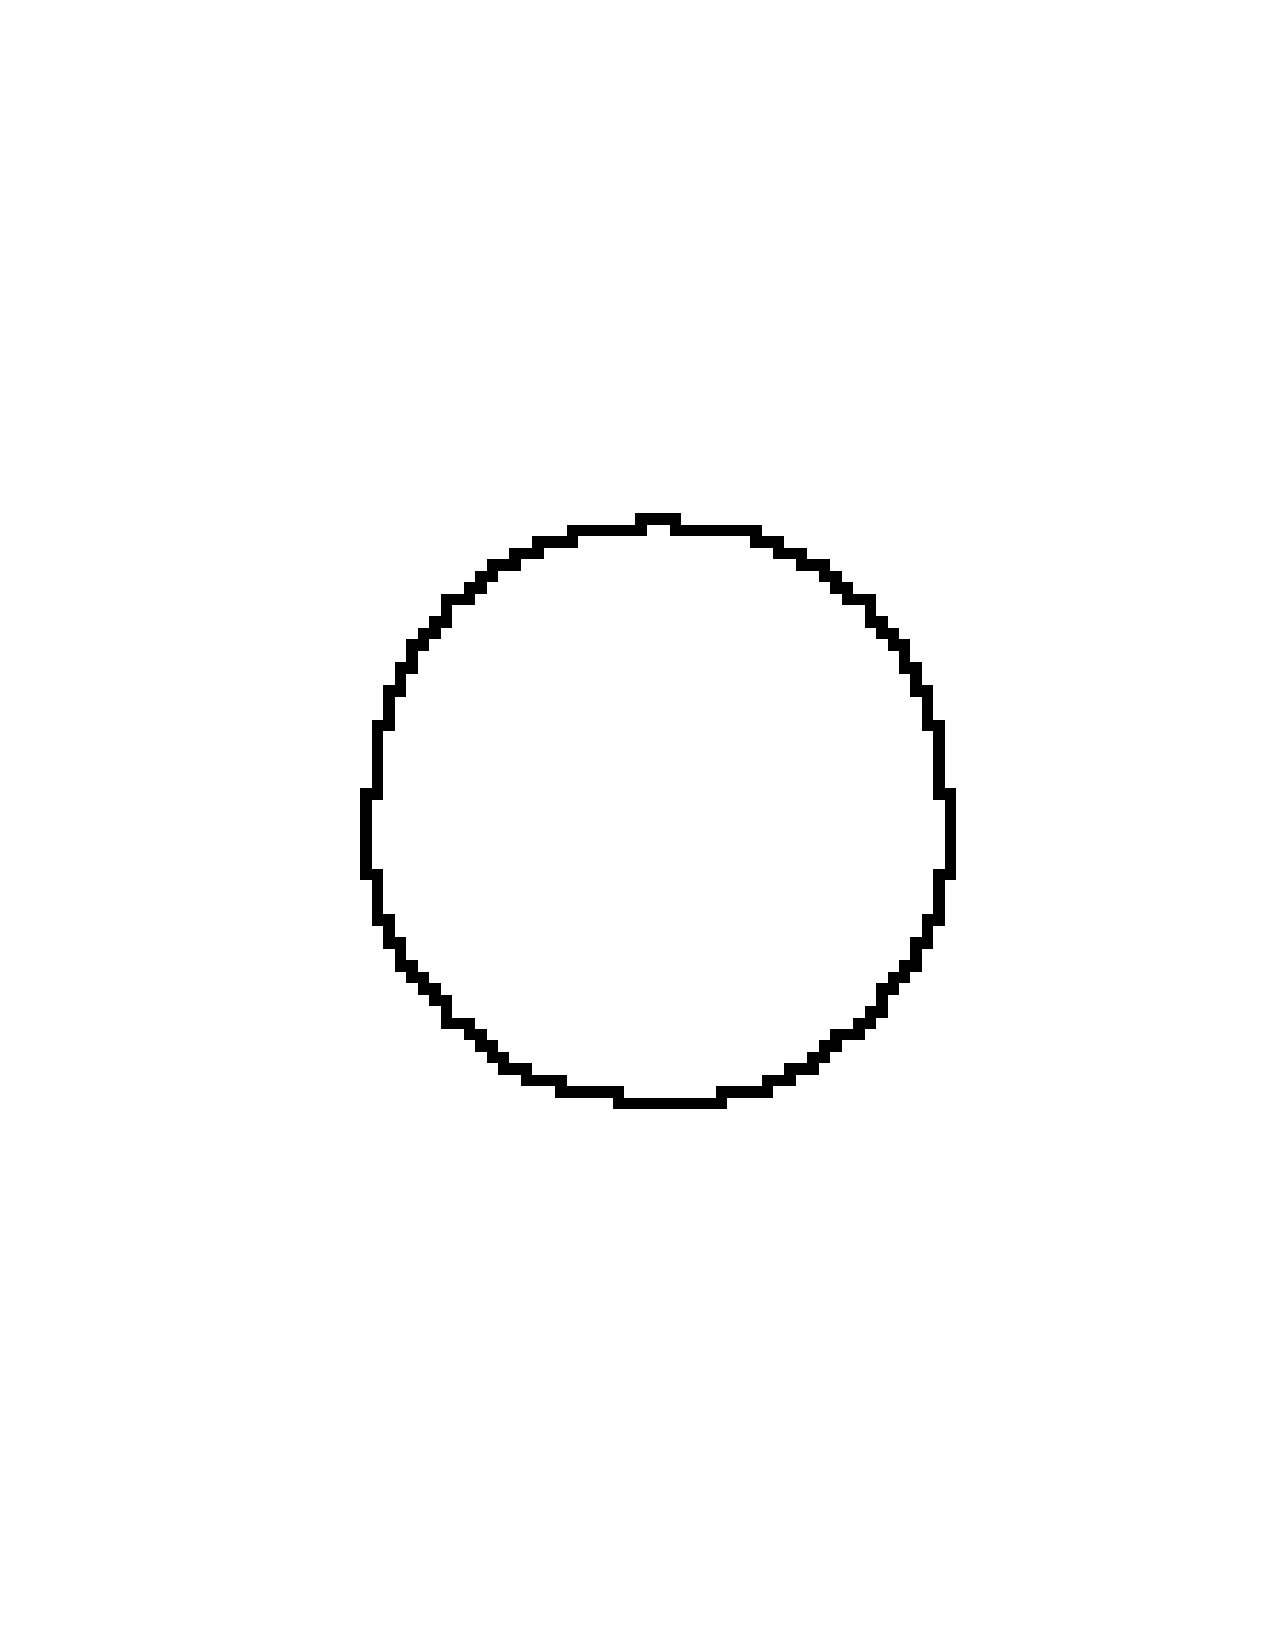
\includegraphics[width=.5\linewidth]{../samples/ring_k3m} 
    \caption{K3M} 
    \vspace{4ex}
  \end{minipage} 
\end{figure}
\FloatBarrier

\par
Pierścień jako figura zamknięta, w porównaniu do koła czy prostokąta, które mogą być po prostu fragmentami lub punktami "grubego" odcinka czy krzywej, zachowuje się dobrze pod wpływem tych programów. Nie jest to raczej zbyt pasjonujący przypadek, choć warto zauważyć, że K3M zostawia grubszy szkielet niż KMM - kwestia zachowania kątów prostych.

\begin{figure}[!ht] 
  \caption{Plama}
  \label{ fig7} 
  \begin{minipage}[b]{0.5\linewidth}
    \centering
    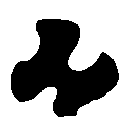
\includegraphics[width=.5\linewidth]{../images/blob} 
    \caption{Obraz wejściowy} 
    \vspace{4ex}
  \end{minipage}%%
  \begin{minipage}[b]{0.5\linewidth}
    \centering
    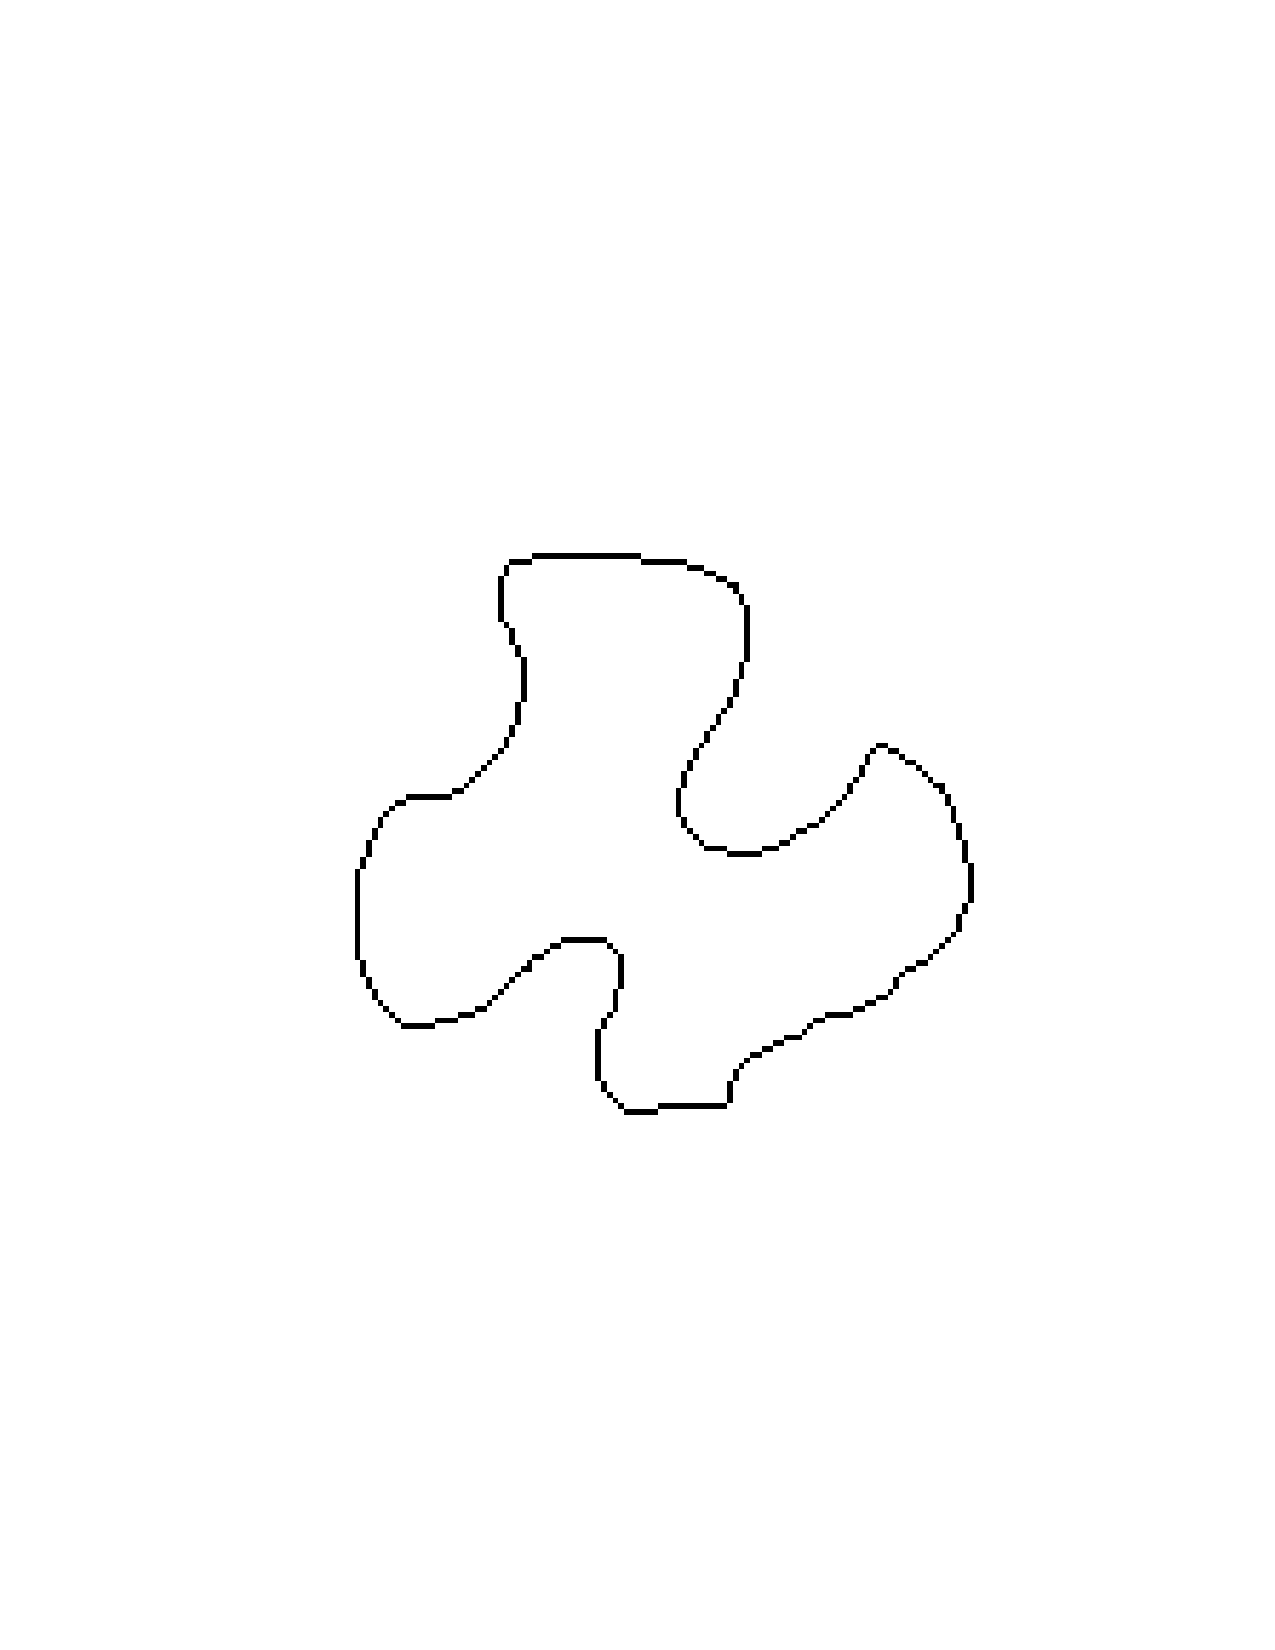
\includegraphics[width=.5\linewidth]{../samples/blob_kmm_contour} 
    \caption{KMM - kontur} 
    \vspace{4ex}
  \end{minipage} 
  \begin{minipage}[b]{0.5\linewidth}
    \centering
    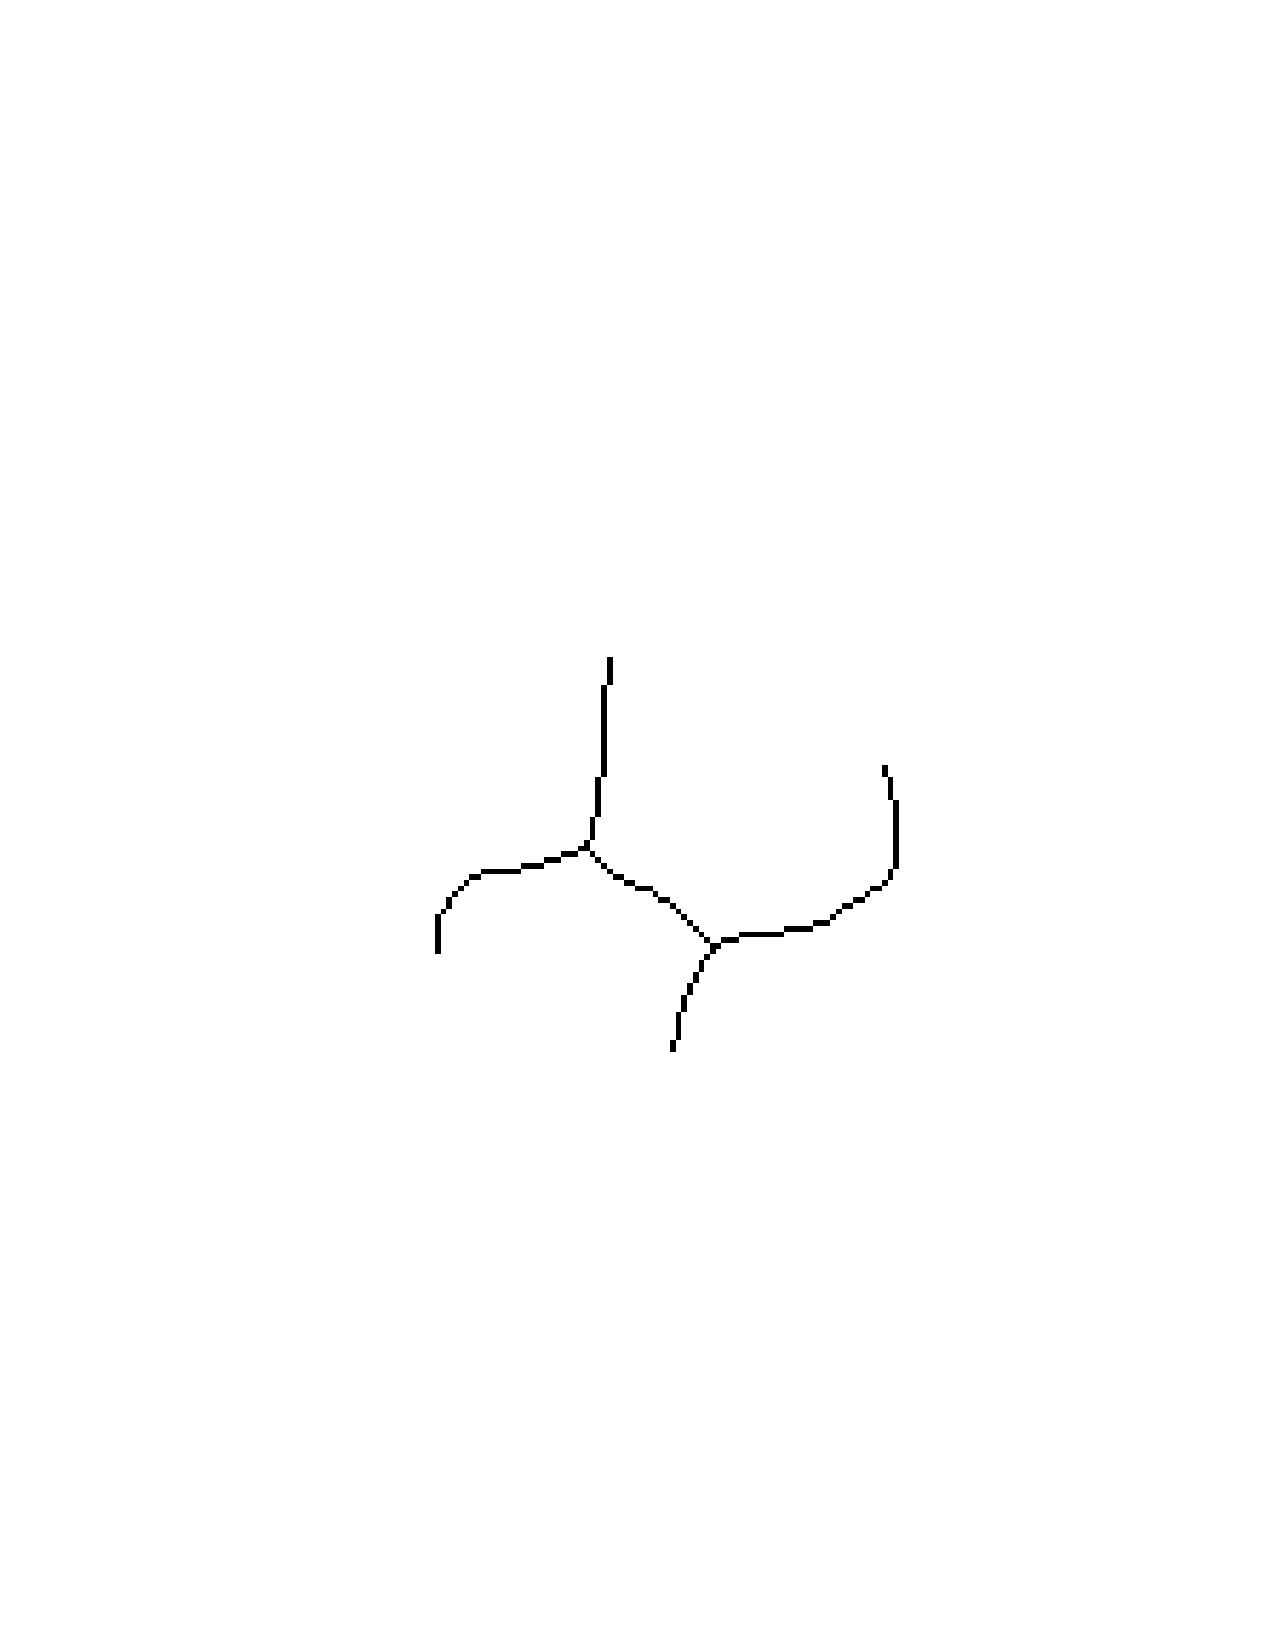
\includegraphics[width=.5\linewidth]{../samples/blob_kmm} 
    \caption{KMM} 
    \vspace{4ex}
  \end{minipage}%% 
  \begin{minipage}[b]{0.5\linewidth}
    \centering
    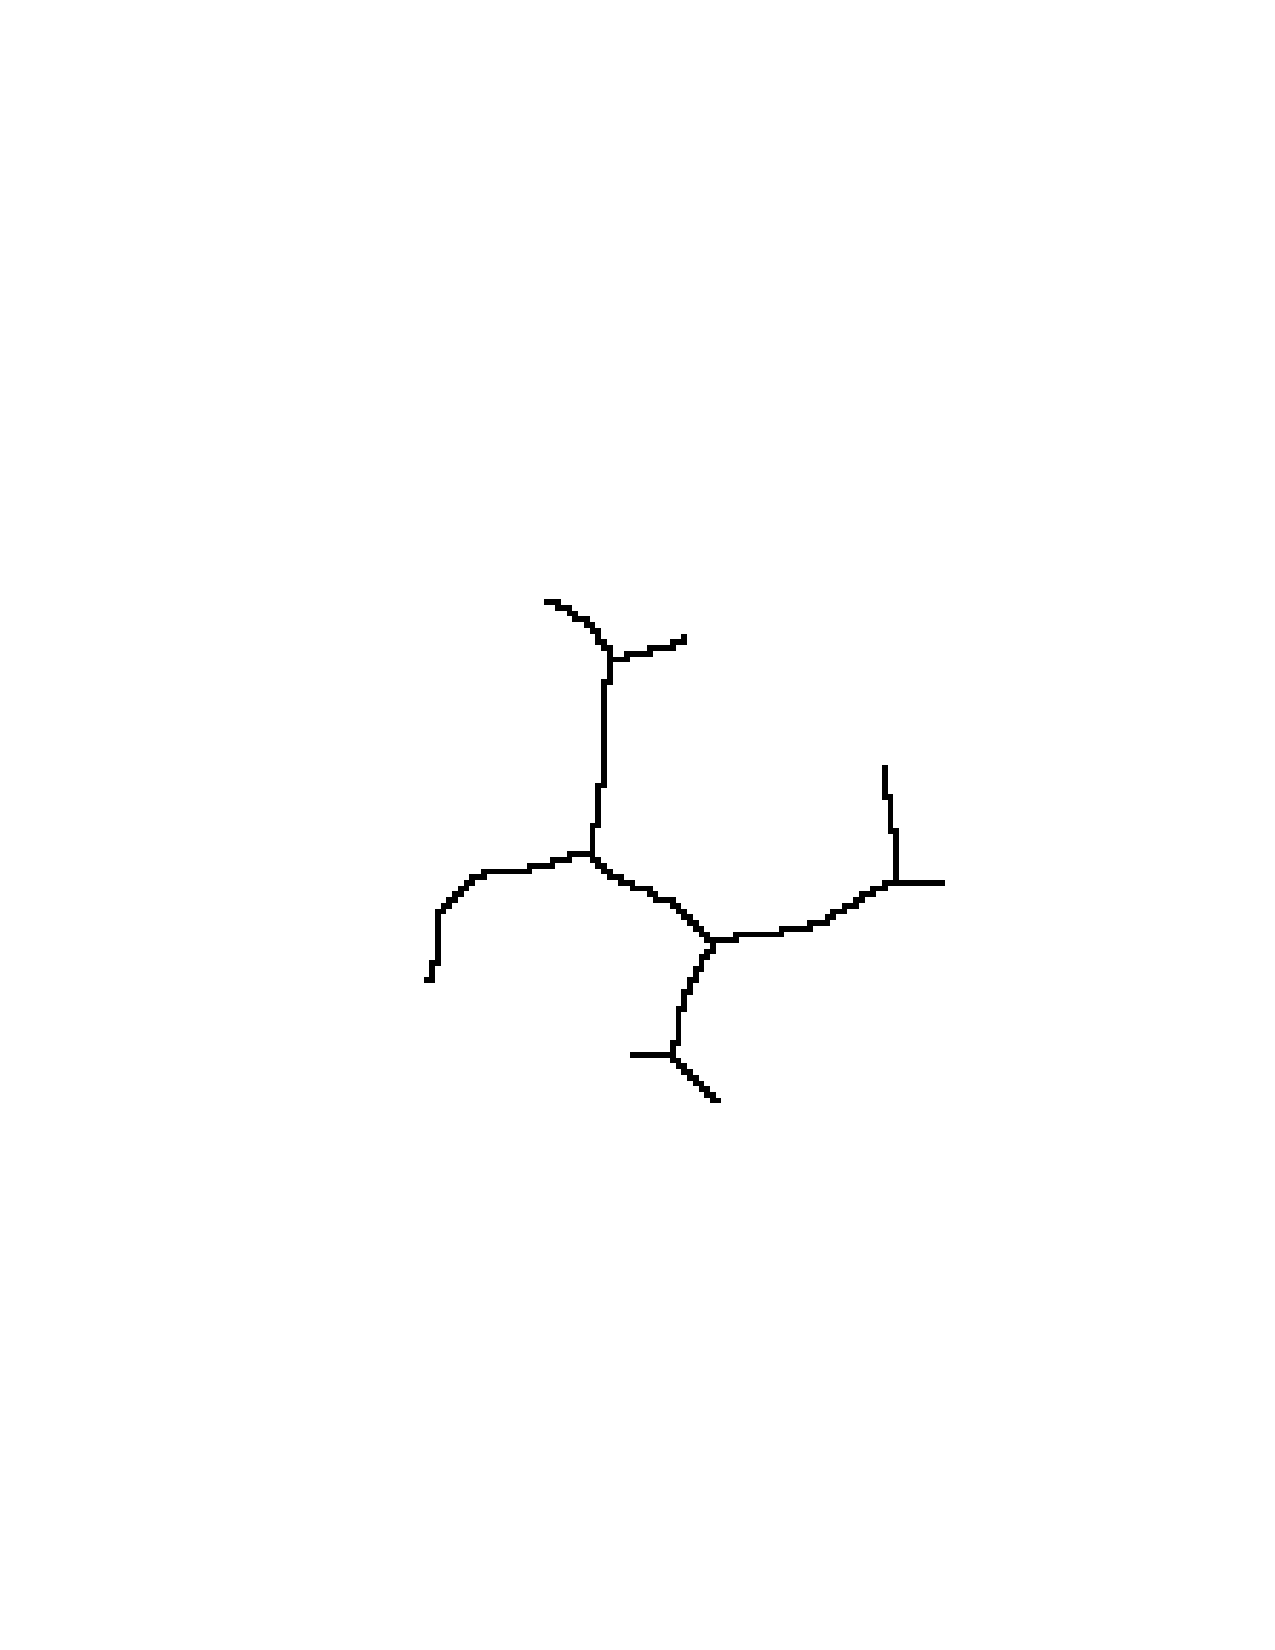
\includegraphics[width=.5\linewidth]{../samples/blob_k3m} 
    \caption{K3M} 
    \vspace{4ex}
  \end{minipage} 
\end{figure}
\FloatBarrier

\par
Ten przykład dobrze ilustruje jak K3M zdecydowanie bardziej stara się wyznaczyć szkielet, który lepiej rozpina kształt niż KMM. Z drugiej strony nie musi to być działanie pożądane - czy potrzebujemy tych dodatkowych gałązek w szkielecie plamy? To pewnie zależy od przypadku.

\begin{figure}[!ht] 
  \caption{Obrazek}
  \label{ fig7} 
  \begin{minipage}[b]{0.5\linewidth}
    \centering
    
\includegraphics[width=.5\linewidth]{../images/sample1} 
    \caption{Obraz wejściowy} 
    \vspace{4ex}
  \end{minipage}%%
  \begin{minipage}[b]{0.5\linewidth}
    \centering
    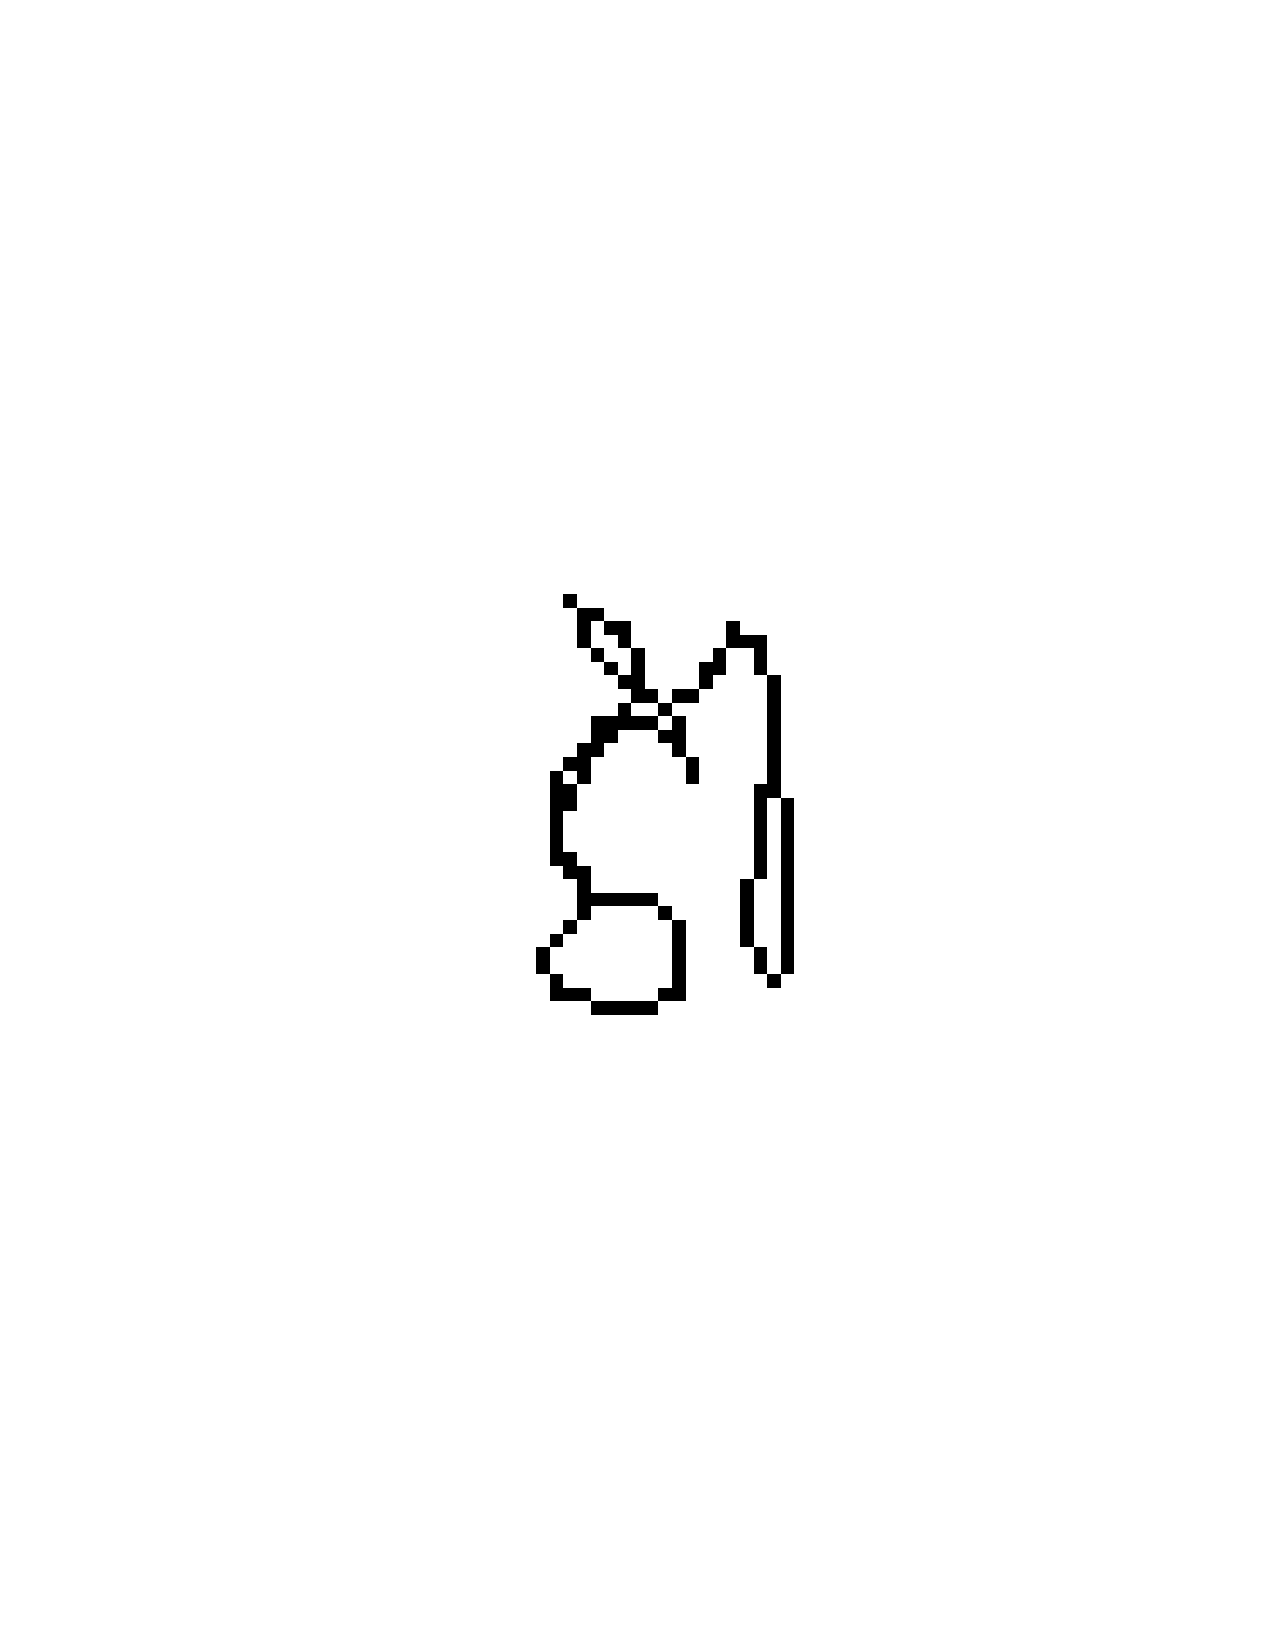
\includegraphics[width=.5\linewidth]{../samples/sample1_kmm_contour} 
    \caption{KMM - kontur} 
    \vspace{4ex}
  \end{minipage} 
  \begin{minipage}[b]{0.5\linewidth}
    \centering
    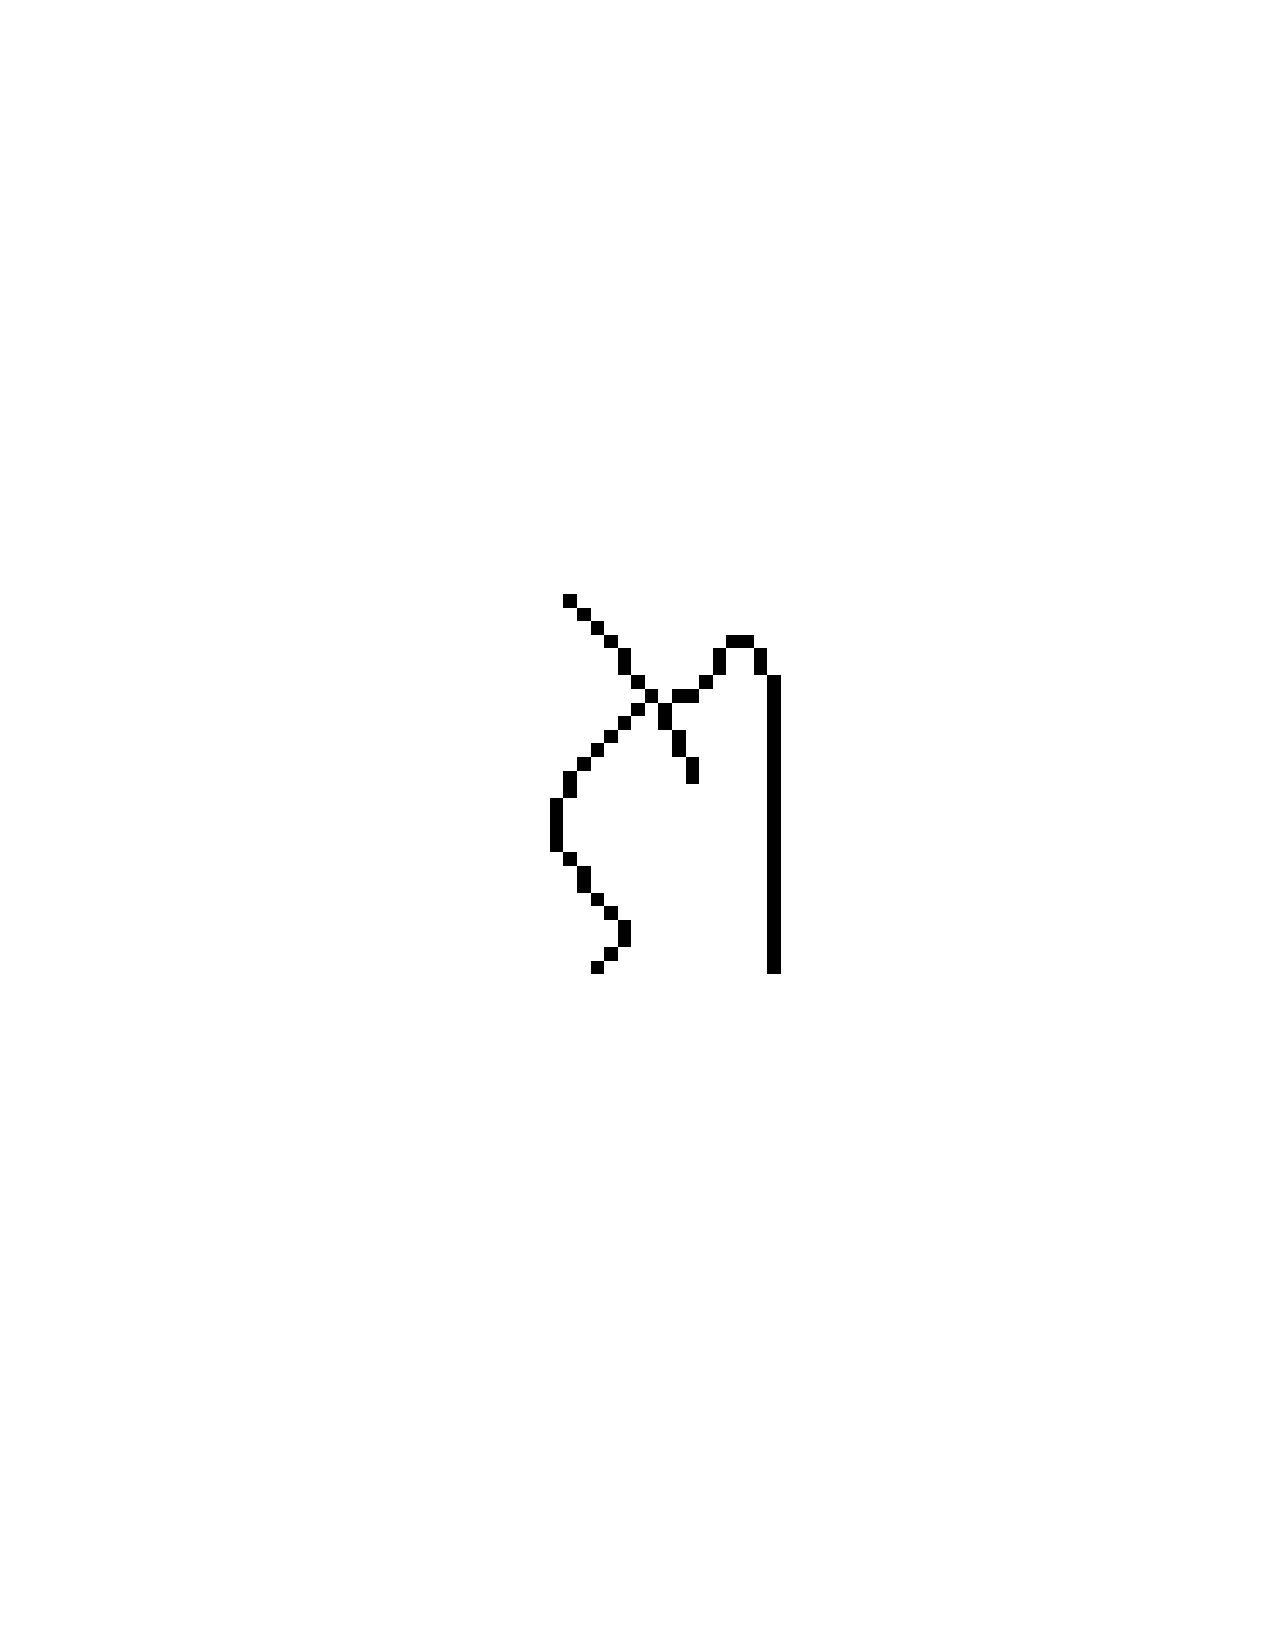
\includegraphics[width=.5\linewidth]{../samples/sample1_kmm} 
    \caption{KMM} 
    \vspace{4ex}
  \end{minipage}%% 
  \begin{minipage}[b]{0.5\linewidth}
    \centering
    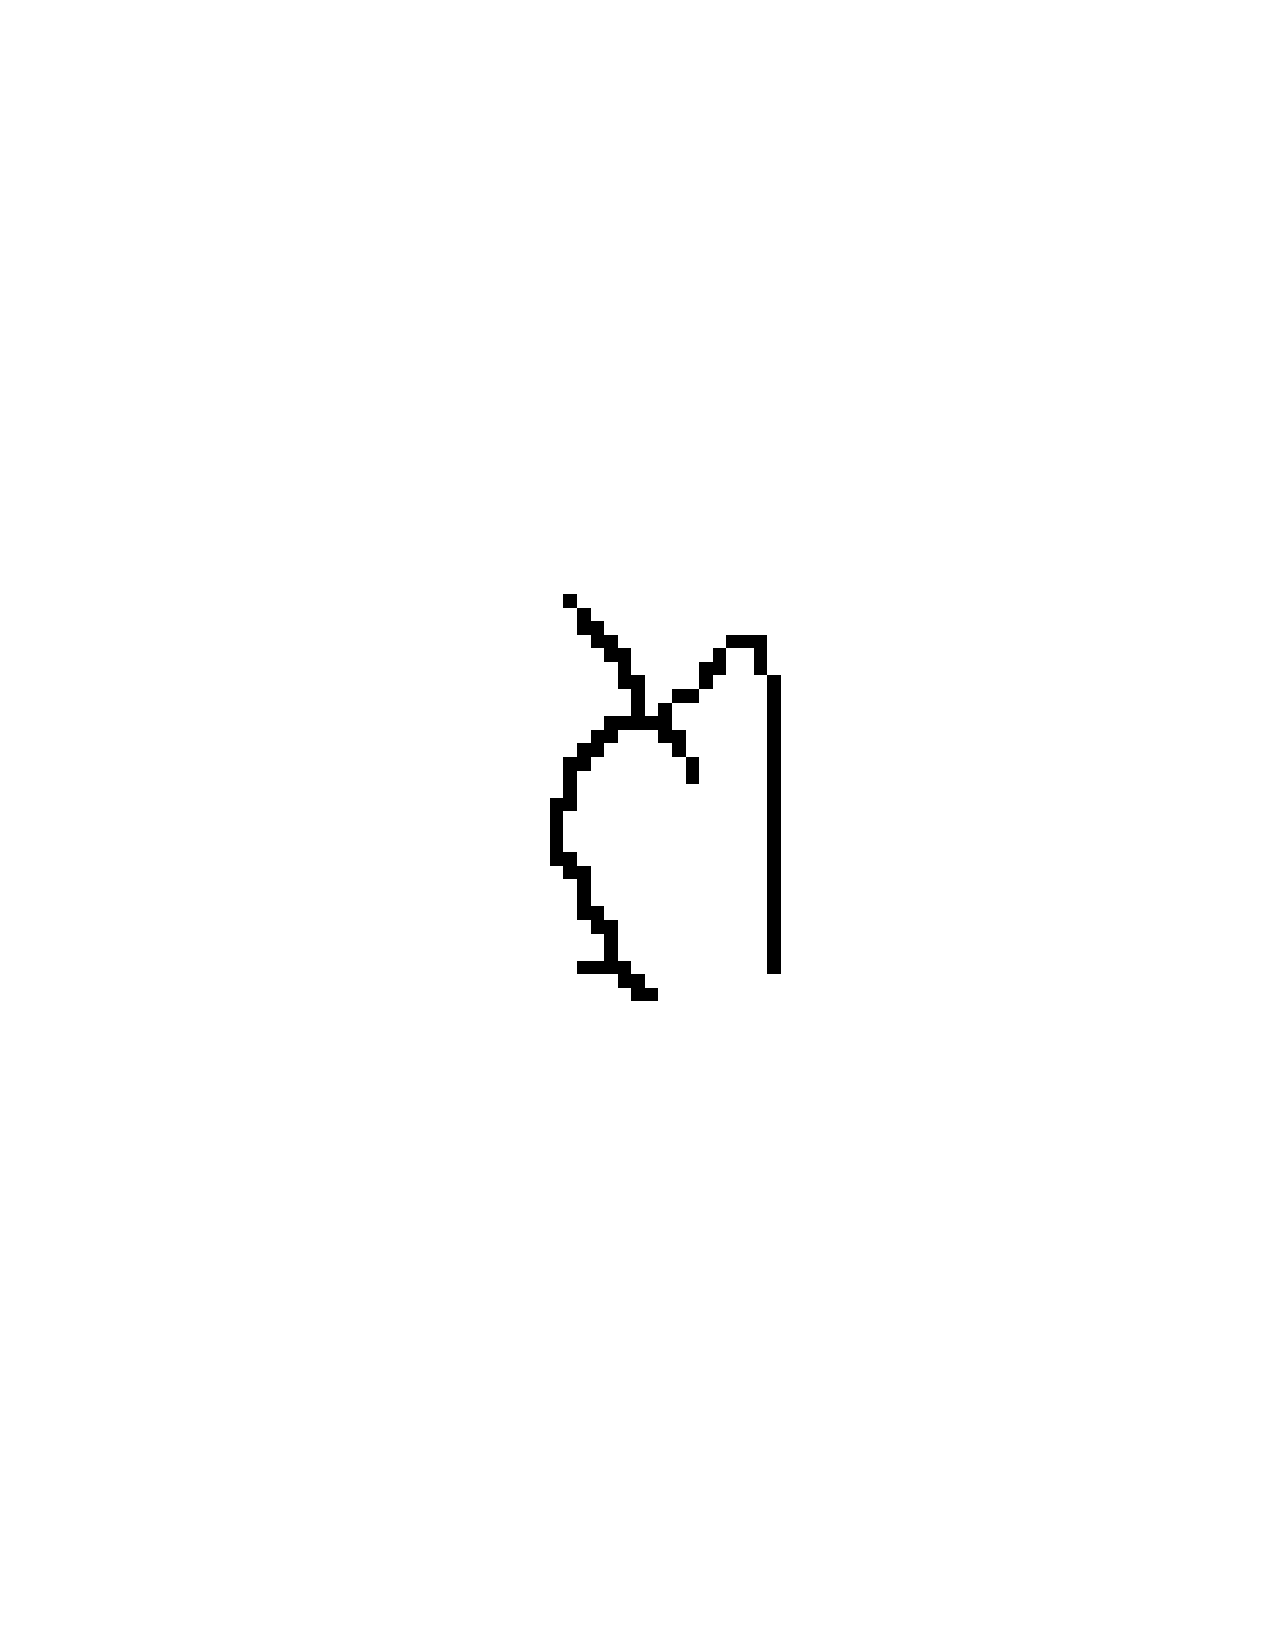
\includegraphics[width=.5\linewidth]{../samples/sample1_k3m} 
    \caption{K3M} 
    \vspace{4ex}
  \end{minipage} 
\end{figure}
\FloatBarrier

\par
To nieskomplikowany obrazek z kilkoma interesującymi punktami. Posiada większą plamę czerni, jakiś dłuższy kształt, jakiś pochyły kształt i kilka połączeń. Dobrze tu widać, że K3M zostawia bardziej kanciasty szkielet. Ponadto znów widać, że w przypadku rozległego, okrągłego kształtu algorytmy nie są zgodne co do zachowania.

\begin{figure}[!ht] 
  \caption{Tekst maszynowy}
  \label{ fig7} 
  \begin{minipage}[b]{0.5\linewidth}
    \centering
    
\includegraphics[width=.5\linewidth]{../images/text} 
    \caption{Obraz wejściowy} 
    \vspace{4ex}
  \end{minipage}%%
  \begin{minipage}[b]{0.5\linewidth}
    \centering
    
\includegraphics[width=.5\linewidth]{../samples/text_kmm_contour} 
    \caption{KMM - kontur} 
    \vspace{4ex}
  \end{minipage} 
  \begin{minipage}[b]{0.5\linewidth}
    \centering
    
\includegraphics[width=.5\linewidth]{../samples/text_kmm} 
    \caption{KMM} 
    \vspace{4ex}
  \end{minipage}%% 
  \begin{minipage}[b]{0.5\linewidth}
    \centering
    
\includegraphics[width=.5\linewidth]{../samples/text_k3m} 
    \caption{K3M} 
    \vspace{4ex}
  \end{minipage} 
\end{figure}
\FloatBarrier

\par
Pismo maszynowe nie jest szczególnie fascynujące przy ścienianiu, ale widać, że efekty są pożądane.

\begin{figure}[!ht] 
  \caption{Pismo odręczne}
  \label{ fig7} 
  \begin{minipage}[b]{0.5\linewidth}
    \centering
    
\includegraphics[width=.5\linewidth]{../images/handwritten} 
    \caption{Obraz wejściowy} 
    \vspace{4ex}
  \end{minipage}%%
  \begin{minipage}[b]{0.5\linewidth}
    \centering
    
\includegraphics[width=.5\linewidth]{../samples/handwritten_kmm_contour} 
    \caption{KMM - kontur} 
    \vspace{4ex}
  \end{minipage} 
  \begin{minipage}[b]{0.5\linewidth}
    \centering
    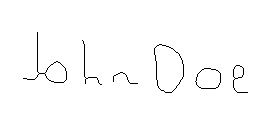
\includegraphics[width=.5\linewidth]{../samples/handwritten_kmm} 
    \caption{KMM} 
    \vspace{4ex}
  \end{minipage}%% 
  \begin{minipage}[b]{0.5\linewidth}
    \centering
    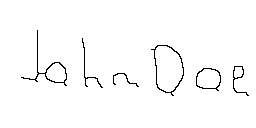
\includegraphics[width=.5\linewidth]{../samples/handwritten_k3m} 
    \caption{K3M} 
    \vspace{4ex}
  \end{minipage} 
\end{figure}
\FloatBarrier

\par
Ostatni już przykład, pismo odręczne, jest chyba najbardziej interesujący i jedyny praktyczny. Pokazuje się tu to, o czym była mowa wyżej - K3M pozostawia gałązki pod kątem 135\degree. Ciekawie też wypadło połączenie liter \textit{J} i \textit{O}.

\section{Źródła}
\begin{enumerate}
\item K. Saeed, M. Rybnik, M. Tabedzki, \\ "Implementation and Advanced Results 
on the Non-Interrupted Skeletonization Algorithm", \\  -- \url{http://aragorn.pb.bialystok.pl/~zspinfo/arts/2001\%20CAIP.pdf}
\item K. Saeed, M. Tabędzki, M. Rybnik, M. Adamski, \\ "K3M: A UNIVERSAL ALGORITHM FOR IMAGE SKELETONIZATION AND A REVIEW OF THINNING TECHNIQUES", \\ Int. J. Appl. Math. Comput. Sci., 2010, Vol. 20, No. 2, 317–335
DOI: 10.2478/v10006-010-0024-4 \\ -- \url{http://matwbn.icm.edu.pl/ksiazki/amc/amc20/amc2029.pdf}
\end{enumerate}

\section{Kod źródłowy}

\subsection{KMM}
\centering
\lstinputlisting[language=Octave,
numbers=left, 
breaklines=true, 
caption={Kod źródłowy KMM (Octave/Matlab)},
basicstyle=\footnotesize]{../scripts/kmm.m}


\subsection{K3M}
\centering
\lstinputlisting[language=Octave,
numbers=left, 
breaklines=true, 
caption={Kod źródłowy K3M (Octave/Matlab)},
basicstyle=\footnotesize]{../scripts/k3m.m}

\end{document}